\documentclass[12pt]{article}
% \usepackage[utf8]{vietnam}
%for times new roman font
% \usepackage{times}
% \usepackage{fourier}
\usepackage[T1]{fontenc}
\usepackage{palatino}

% \newfontfamily\cfont{Caladea}
% \newfontfamily\vfont{Verdana}

\usepackage{a4wide,amssymb,epsfig,latexsym,multicol,array,hhline,fancyhdr}
\usepackage{amsmath}
\usepackage{newtxmath}
\usepackage{lastpage}
\usepackage{minted}
%\usepackage[lined,boxed,commentsnumbered]{algorithm2e}
\usepackage{enumerate}
\usepackage{float}
\usepackage[shortlabels]{enumitem}

\usepackage{color}
\usepackage{subcaption}
\usepackage{graphicx}							% Standard graphics package
\usepackage{array}
\usepackage{tabularx, caption}
\usepackage{multirow}
\usepackage{multicol}
\usepackage{rotating}
\usepackage[most]{tcolorbox}
\usepackage{graphics}
\usepackage{geometry}
\usepackage{listings}
\usepackage{xcolor}
\usepackage[stable]{footmisc}

% For algorithm
\usepackage{algorithm}
\usepackage{algpseudocode}
\usepackage{hyperref}

\usepackage{setspace}
\usepackage{epsfig}
\usepackage{bm}
\usepackage{tikz}
\usepackage{float}
\usepackage{adjustbox}
\usetikzlibrary{arrows,snakes,backgrounds}
\usepackage{hyperref}
\hypersetup{
	colorlinks,
	linktoc=all,
	linkcolor=blue,
	citecolor=black,
	urlcolor=black,
}

\usepackage{array}
\usepackage{makecell}

\renewcommand\theadalign{bc}
\renewcommand\theadfont{\bfseries}
\renewcommand\theadgape{\Gape[4pt]}
\renewcommand\cellgape{\Gape[4pt]}
%\hypersetup{urlcolor=blue,linkcolor=black,citecolor=black,colorlinks=true} 
%\usepackage{pstcol} 								% PSTricks with the standard color package
\newcommand*\circled[1]{\tikz[baseline=(char.base)]{
		\node[shape=circle,draw,inner sep=0.1pt] (char) {#1};}}
\newtheorem{theorem}{{\bf Theorem}}
\newtheorem{property}{{\bf Property}}
\newtheorem{proposition}{{\bf Proposition}}
\newtheorem{corollary}[proposition]{{\bf Corollary}}
\newtheorem{lemma}[proposition]{{\bf Lemma}}

\AtBeginDocument{\renewcommand*\contentsname{Contents}}
\AtBeginDocument{\renewcommand*\refname{References}}
%\usepackage{fancyhdr}
\setlength{\headheight}{40pt}
\pagestyle{fancy}
\fancyhead{} % clear all header fields
\fancyhead[L]{
 \begin{tabular}{rl}
    \begin{picture}(25,15)(0,0)
    \put(0,-8){
\includegraphics[width=8mm, height=8mm]{hcmut.png}}
    %\put(0,-8){\epsfig{width=10mm,figure=hcmut.eps}}
   \end{picture}&
	%
\includegraphics[width=8mm, height=8mm]{hcmut.png} & %
	\begin{tabular}{l}
		\text{\ttfamily University of Technology, Ho Chi Minh City}\\
		\text{\ttfamily Faculty of Computer Science and Engineering}
	\end{tabular} 	
 \end{tabular}
}
\fancyhead[R]{
	\begin{tabular}{l}
		\tiny \bf \\
		\tiny \bf 
	\end{tabular}  }
\fancyfoot{} % clear all footer fields
\fancyfoot[L]{\scriptsize \ttfamily Assignment for Advanced Programming - Academic year 2023 - 2024}
\fancyfoot[R]{\scriptsize \ttfamily Page {\thepage}/\pageref{LastPage}}
\renewcommand{\headrulewidth}{0.3pt}
\renewcommand{\footrulewidth}{0.3pt}

\newcommand{\code}[1]{\texttt{#1}}

\definecolor{gray}{RGB}{247, 247, 247}
%\definecolor{pr}{RGB}{0, 153, 115}
\definecolor{pr}{RGB}{0, 0, 102}
\definecolor{dpr}{RGB}{0, 102, 102}
\definecolor{fb}{RGB}{0, 153, 115}
\definecolor{co}{RGB}{113, 148, 218}
\definecolor{bapro}{RGB}{250, 250, 250}

\definecolor{codegreen}{rgb}{0,0.6,0}
\definecolor{codegray}{rgb}{0.5,0.5,0.5}
\definecolor{codepurple}{rgb}{0.58,0,0.82}
\definecolor{backcolour}{rgb}{0.95,0.95,0.92}

\lstdefinestyle{mystyle}{
  backgroundcolor=\color{backcolour}, commentstyle=\color{codegreen},
  keywordstyle=\color{magenta},
  numberstyle=\tiny\color{codegray},
  stringstyle=\color{codepurple},
  basicstyle=\ttfamily\footnotesize,
  breakatwhitespace=false,         
  breaklines=true,                 
  captionpos=b,                    
  keepspaces=true,                 
  numbers=left,                    
  numbersep=5pt,                  
  showspaces=false,                
  showstringspaces=false,
  showtabs=false,                  
  tabsize=2
}

\lstset{style=mystyle}

\parindent 0pt

%%%
\setcounter{secnumdepth}{4}
\setcounter{tocdepth}{3}
\makeatletter
\newcounter {subsubsubsection}[subsubsection]
\renewcommand\thesubsubsubsection{\thesubsubsection .\@alph\c@subsubsubsection}
\newcommand\subsubsubsection{\@startsection{subsubsubsection}{4}{\z@}%
                                     {-3.25ex\@plus -1ex \@minus -.2ex}%
                                     {1.5ex \@plus .2ex}%
                                     {\normalfont\normalsize\bfseries}}
\newcommand*\l@subsubsubsection{\@dottedtocline{3}{10.0em}{4.1em}}
\newcommand*{\subsubsubsectionmark}[1]{}
\makeatother

\definecolor{gray}{RGB}{247, 247, 247}
\definecolor{pr}{RGB}{0, 32, 128}
\definecolor{bapr}{RGB}{0, 32, 128}
\definecolor{l}{RGB}{102, 153, 204}
\colorlet{co}{cyan!70!black}
\definecolor{codegreen}{rgb}{0,0.6,0}
\definecolor{codegray}{rgb}{0.5,0.5,0.5}
\definecolor{codepurple}{rgb}{0.58,0,0.82}
\definecolor{backcolour}{rgb}{0.95,0.95,0.92}

\newtcolorbox{cmt}[1]
{
	boxrule=0pt,
	boxsep=0pt,
	colback=white,
	detach title,
	before upper={\tcbtitle \ },
	fonttitle=\bfseries,
	coltitle=black,
	title=#1,
	% borderline west={2.5pt}{0pt}{black},
        toprule=0.8pt,
	bottomrule=0.8pt,
	leftrule=0.8pt,
	rightrule=0.8pt,
        arc=0pt,outer arc=0pt
	enhanced jigsaw,
	before skip=10pt,
	after skip=10pt,
	breakable,
}

\newtcolorbox{pro}[1]
{
	boxrule=1pt,
	boxsep=1pt,
	colback=white,
	attach boxed title to top left ={xshift=2mm,yshift=-3mm,yshifttext=-2mm},
	boxed title style={size=small,colframe=white},
	fonttitle=\bfseries\sffamily,
	coltitle=white,
	colbacktitle=bapr,
	title=#1,
	colframe=pr,
	toprule=0.8pt,
	bottomrule=0.8pt,
	leftrule=0.8pt,
	rightrule=0.8pt,
	enhanced jigsaw,
	before skip=10pt,
	after skip=10pt,
	breakable,
}

\lstdefinestyle{mystyle}{
  % backgroundcolor=\color{white}, 
  % commentstyle=\color{codegray},
  % keywordstyle=\color{black},
  % numberstyle=\tiny\color{black},
  % stringstyle=\color{black},
  % basicstyle=\ttfamily\scriptsize,
  % breakatwhitespace=false,         
  % breaklines=true,                 
  % captionpos=b,                    
  % keepspaces=true,                 
  % numbers=left,                    
  % numbersep=5pt,                  
  % showspaces=false,                
  % showstringspaces=false,
  % showtabs=false,                  
  % tabsize=2
  backgroundcolor=\color{backcolour}, commentstyle=\color{codegreen},
  keywordstyle=\color{magenta},
  numberstyle=\tiny\color{codegray},
  stringstyle=\color{codepurple},
  basicstyle=\ttfamily\footnotesize,
  breakatwhitespace=false,         
  breaklines=true,                 
  captionpos=b,                    
  keepspaces=true,                 
  numbers=left,                    
  numbersep=5pt,                  
  showspaces=false,                
  showstringspaces=false,
  showtabs=false,                  
  tabsize=2
}

\lstset{style=mystyle}
% Set TOC depth
\setcounter{tocdepth}{2}

\begin{document}

\begin{titlepage}
\begin{center}
VIETNAM NATIONAL UNIVERSITY, HO CHI MINH CITY \\
UNIVERSITY OF TECHNOLOGY \\
FACULTY OF COMPUTER SCIENCE AND ENGINEERING
\end{center}

\vspace{1cm}

\begin{figure}[h!]
\begin{center}

\includegraphics[width=5cm]{hcmut.png}
\end{center}
\end{figure}

\vspace{1cm}


\begin{center}
\begin{tabular}{c}
\multicolumn{1}{l}{\textbf{{\Large ADVANCED PROGRAMMING (CO2039)}}}\\
~~\\
\hline
\\
\multicolumn{1}{l}{\textbf{{\Large Assignment}}}\\
\\
\textbf{{\huge Functional Programming in Python}}
\\[0.8em]
\hline
\end{tabular}
\end{center}

\vspace{1cm}

\begin{table}[h]
\begin{tabular}{rrll}
\hspace{5 cm} & Advisor: & Truong Tuan Anh & \\
& & Phan Duy Han \\
& Students: & Nguyen Tien Hung - 2252280\\
\end{tabular}
\end{table}

\begin{center}
{\footnotesize HO CHI MINH CITY, MAY 2024}
\end{center}
\end{titlepage}


%\thispagestyle{empty}

\newpage
\tableofcontents
\newpage


\section{Introduction about Functional Programming}
\subsection{Definitions}
Functional programming is a declarative programming paradigm style where one applies pure functions in sequence to solve complex problems. Functions take an input value and produce an output value without being affected by the program. Functional programming mainly focuses on what to solve and uses expressions instead of statements. Functional programming excels mostly at mathematical functions where the values don’t have any correlation and doesn’t make use of concepts like shared state and mutable data used in object-oriented programming.
\subsection{Functional Programming Concepts}
Functional programming is built with various core concepts which we will explore below:
\begin{itemize}
    \item \textbf{First-class functions:} First-class functions in functional programming are treated as data type variables and can be used like any other variables. These first-class variables can be passed to functions as parameters, or stored in data structures.
    \item \textbf{Recursion:} Unlike object-oriented programming, functional programming doesn’t make use of “while” or ”for” loops or “if-else” statements. Functional programs avoid constructions that create different outputs on every execution. Instead, recursive functions call themselves repeatedly until they reach the desired state or solution known as the base case.
    \item \textbf{Immutability:} In functional programming, we can’t modify a variable after being created. The reason for this is that we would want to maintain the program's state throughout the runtime of the program. It is best practice to program each function to produce the same result irrespective of the program's state. This means that when we create a variable and assign a value, we can run the program with ease fully knowing that the value of the variables will remain constant and can never change.
    \item \textbf{Pure functions:} Pure functions form the foundation of functional programming and have two major properties: They produce the same output if the given input is the same, They have no side effects.\\
    Pure functions work well with immutable values as they describe how inputs relate to outputs in declarative programs. Because pure functions are independent this means that they are reusable, easy to organize, and debug, making programs flexibly and adaptable to changes. Another advantage of using pure functions is memoization. This is when we cache and reuse the results after computing the outputs from the given inputs.
    \item \textbf{High order functions:} A function that accepts other functions as parameters or returns functions as outputs is called a high order function. This process applies a function to its parameters at each iteration while returning a new function that accepts the next parameter.
\end{itemize}

\begin{figure}[h!]
\begin{center}
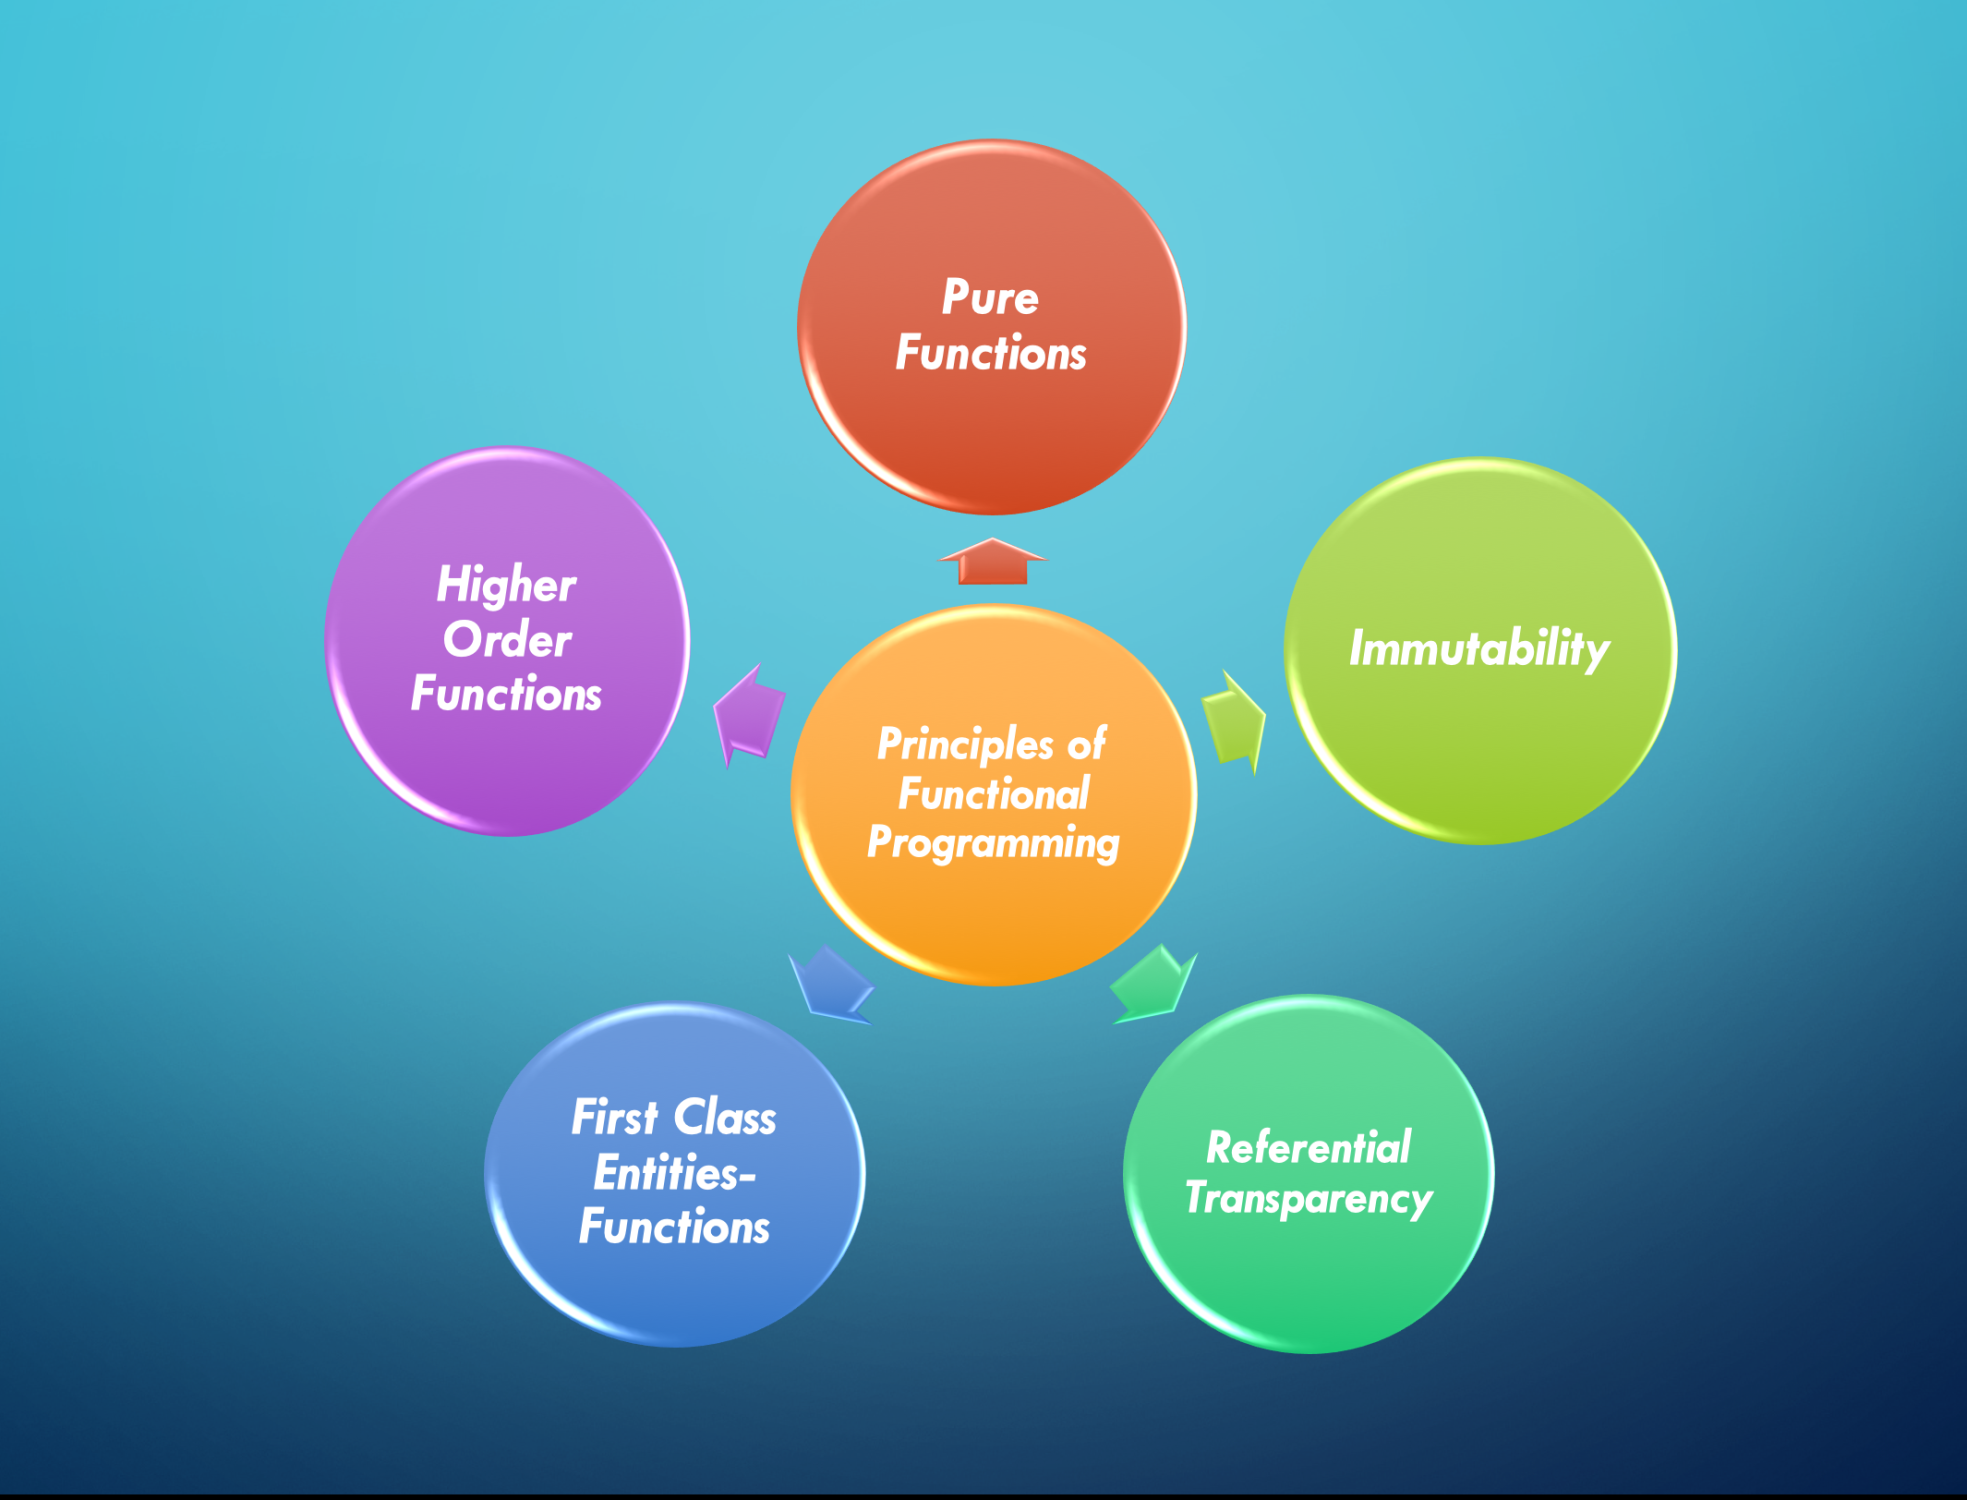
\includegraphics[width=13cm]{Intro1.png}\\
Mindmap Concepts of Functional Programming
\end{center}
\end{figure}

\subsection{Advantages of functional programming}
Functional programming (FP) offers numerous advantages that stem from its core principles and paradigms. Here are some of the key benefits:
\begin{itemize}
    \item \textbf{Easy to debug:} Since pure functions produce the same output as the given input, this means they aren’t any changes or any other hidden output produced. Functional programming functions are immutable, this also means that it’s easier to check for errors in code faster.
    \item \textbf{Lazy evaluation:} Functional programming adopts the lazy evaluation concept, whereby the computations are only evaluated the moment they are needed. This gives programs the ability to reuse results produced from previous computations.
    \item \textbf{Supports parallel programming:} Because functional programming uses immutable variables, creating parallel programs is easy as they reduce the amount of change within the program. Each function only has to deal with an input value and have the guarantee that the program state will remain constant.
    \item \textbf{Easy to read:} Functions in functional programming are easy to read and understand. Since functions are treated as values, immutable, and can be passed as parameters, it is easier to understand the codebase and purpose.
    \item \textbf{Efficient:} Since functional programs don’t rely on any external sources or variables to function, they are easily reusable across the program. This makes them more efficient as there isn’t extra computation needed to source the programs or run operations on runtime.
\end{itemize}
\subsection{Drawbacks of Functional Programming}
While functional programming (FP) offers many advantages, it also comes with some drawbacks that can make it challenging to adopt or less suitable for certain types of tasks. Here are some of the key disadvantages:

\begin{itemize}
    \item \textbf{Terminology Problems:} Because of its mathematical roots, functional programming has a lot of terminologies that may be difficult to explain to a layman. Terms like “pure functions” can easily scare off people looking to learn more about functional programming.
    \item \textbf{Recursion:} Although recursion is one of the best features in functional programming, it is very expensive to use. Writing recursive functions requires higher memory usage which can be costly.
\end{itemize}

\begin{figure}[h!]
\begin{center}
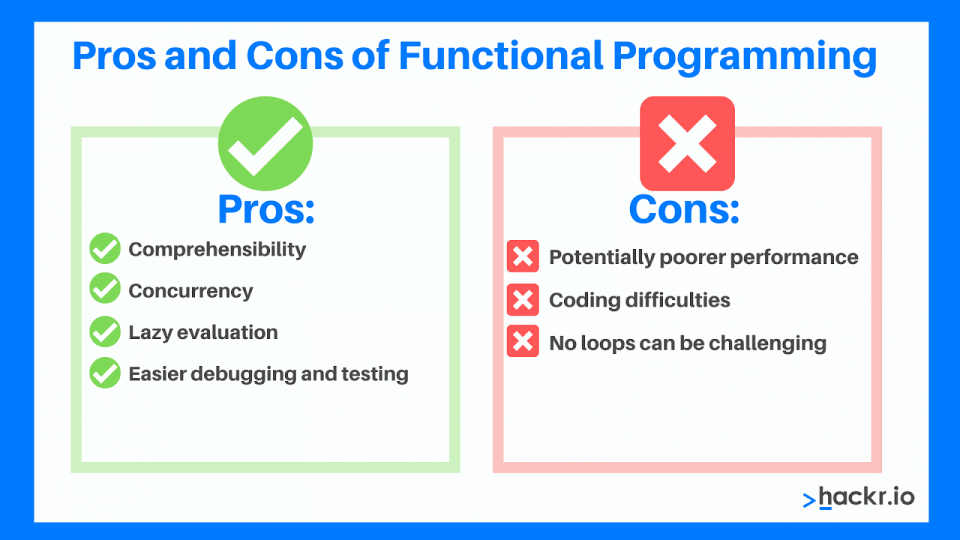
\includegraphics[width=13cm]{Intro2.png}\\
Pros and Cons of Functional Programming
\end{center}
\end{figure}

\subsection{Comparison Functional Programming with another Type Programming}
This semester, our curriculum emphasizes Object-Oriented Programming (OOP), providing us with a solid understanding of its principles and practices. Given this focus, it's an excellent time to delve into a comparative analysis with Functional Programming (FP). By exploring the contrasts and similarities between these two paradigms, we can gain deeper insights into their respective methodologies, advantages, and use cases. This comparison will not only enhance our grasp of OOP but also broaden our overall programming knowledge by highlighting the distinct philosophies that drive FP. As we progress through the semester, examining how OOP and FP approach problems, structure code, and manage data will be both enlightening and beneficial for our development as versatile programmers.

\subsubsection{Definitions of Object Oriented Programming}
Object-Oriented Programming (OOP) is a programming paradigm centered around the concept of objects, which are instances of classes. Classes define the structure and behavior of objects, encapsulating data and functions that operate on the data. OOP promotes principles such as encapsulation, inheritance, and polymorphism, which help in organizing code into modular, reusable, and maintainable components. Encapsulation hides the internal state of objects and only exposes necessary functionalities, ensuring a clear interface. Inheritance allows classes to inherit properties and behaviors from other classes, promoting code reuse. Polymorphism enables objects to be treated as instances of their parent class, allowing for flexible and dynamic code. By modeling real-world entities as objects, OOP makes it easier to design complex software systems with clear relationships and interactions.
\\
\textbf{Therefore, the object is the primary and fundamental unit of OOP programming methodology, and it consists of the following elements:}
\begin{itemize}
    \item Classes and objects make the code clean and streamlined, leading authorized persons to understand it precisely.
    \item A state describing its characteristics and attributes.
    \item Behavior to assess how the object will interact and respond to other objects in code.
\end{itemize}


\begin{figure}[h!]
\begin{center}
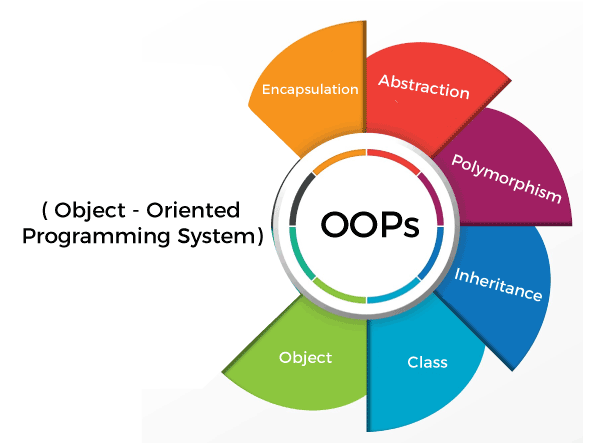
\includegraphics[width=8cm]{Intro3.png}\\
Characteristic of OOP
\end{center}
\end{figure}

In addition, Java, Python, C++, Ruby, and C\# are the most popular and preferred programming languages for crafting an application following the OOP mechanism. These languages use multiple objects to define every operation for inputting, processing, and providing output.

You must be wondering what makes OOP highly considerable, and the answer to this question is its below-listed authentic features:
\begin{itemize}
    \item \textbf{Inheritance:} With this feature, you can inherit the properties of one class to another, including its methods and properties.
    \item \textbf{Polymorphism:} It helps to use a single feature for executing multiple actions through overriding and overloading.
    \item \textbf{Abstraction:} Users utilize this concept to hide unnecessary information and display only relevant details on the interface.
    \item \textbf{Encapsulation:} It aids in hiding the state, behavior, and structure of an object created inside a class and prevents unauthorized access to core components.
\end{itemize}

\begin{figure}[h!]
\begin{center}
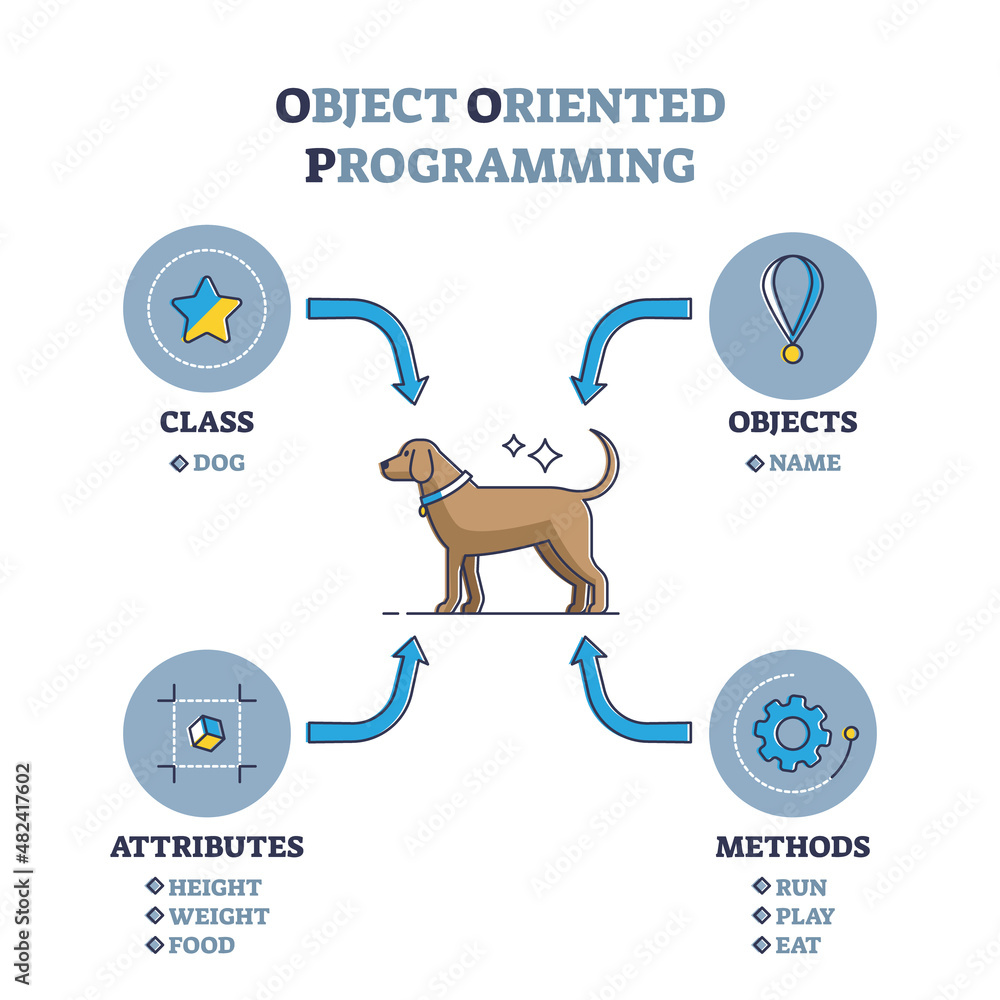
\includegraphics[width=8cm]{Intro4.jpg}\\
Some features of OOP
\end{center}
\end{figure}

\vspace{1cm}

\hspace{7.5em} {\textbf{Object-Oriented Programming vs Functional Programming}}
\begin{center}
\begin{tabular}{ | c | c | c | }
  \hline
  \thead{Basis} & \thead{Object-Oriented Programming} & \thead{Functional Programming}\\
  \hline
  \makecell{\textbf{Programming Model} \\ \textbf{Followed}} &  \makecell{Imperative Model focused on \\ data modeling through \\active dynamic statements}  &  \makecell{ Declarative Model, aiming to define \\logic rather than data flow } \\
  \hline
  \makecell{\textbf{Support for} \\ \textbf{Parallel Programming}} &  \makecell{It doesn’t offer \\ parallel programming}  &  \makecell{ Parallel programming can be \\implemented in the program } \\
  \hline
  \makecell{\textbf{Data Handling}} &  \makecell{Functions effectively \\ with mutable data}  &  \makecell{ Immutable data is \\used for functioning } \\
  \hline
  \makecell{\textbf{Execution Order}} &  \makecell{Only called method in a \\ class can be executed}  &  \makecell{ Functions can be performed \\ in any order } \\
  \hline
  \makecell{\textbf{Utilization}} &  \makecell{Preferred for high input and \\ fewer operation processing}  &  \makecell{ Considered for low input and \\more processing software } \\
  \hline
  \makecell{\textbf{Ease-to-Learn}} &  \makecell{Complex to learn, due to  \\non-modularity as compared to \\Functional Methodology}  &  \makecell{ Simple to learn for both \\freshers and professionals } \\
  \hline
  \makecell{\textbf{Maintainability}} &  \makecell{Effortless maintenance \\ due to classes}  &  \makecell{Difficult to maintain and update} \\
  \hline
  \makecell{\textbf{Implementation}} &  \makecell{Programs can be created \\ straightforwardly}  &  \makecell{ A different functional \\viewpoint is required } \\
  \hline
\end{tabular}
\end{center}

\subsubsection{Advantages of Object-Oriented Programming}
Object-Oriented Programming (OOP) offers several advantages that make it a preferred paradigm for software development. Here are some of the key benefits:

\begin{itemize}
    \item Classes and objects make the code clean and streamlined, leading authorized persons to understand it precisely.
    \item It follows an imperative style, due to which code looks like a set of instructions and leverages to the system to read it faster.
    \item Developers can use objects of developed libraries in a project in other future projects for creating quality software within cost and time constraints.
    \item Large-scale and modular business applications benefit from enhanced security.
    \item Its flawless memory management divides the elements into small parts and helps to reduce junk values during process execution.
\end{itemize}

\subsubsection{Disadvantages of Functional Programming}
Functional Programming (FP) offers many advantages, but it also comes with its own set of challenges and disadvantages. Here are some of the key disadvantages associated with FP:
\begin{itemize}
    \item People used to OOP find it complex to implement recursion functions in code.
    \item More mathematical calculations are performed during development, making the process complicated and increasing effort.
    \item Less documentation is available, making it difficult to learn and identify solutions to complexities in programming.
    \item Sometimes it is not suitable for large projects, as defining more and more functions can create errors, loopholes, and glitches in the final solution.
    \item Graph-based algorithms don’t work properly and run slower as compared to OOP.
\end{itemize}

\subsubsection{When to use, Functional Programming or OOP}
Object-oriented programming focuses on data, whereas functional programming prioritizes operation execution. If your application requires data modeling, you must consider OOP, and if you want efficient task processing, you must prefer functional programming.

\begin{figure}[h!]
\begin{center}
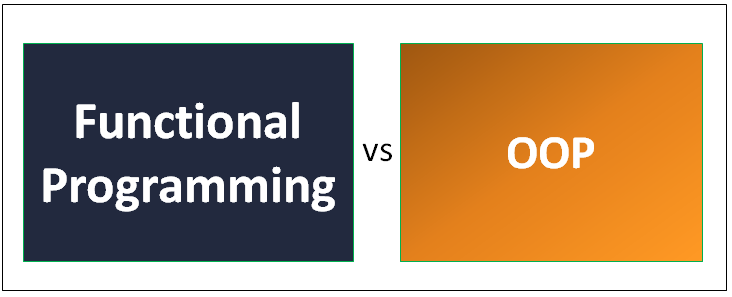
\includegraphics[width=9cm]{Intro5.png}\\
Functional Programming vs OOP
\end{center}
\end{figure}

\subsection{Functional programming languages}
Now as you can imagine not all programming languages support functional programming. Some languages however were designed to be specifically for functional programming, while others do support both functional and object-oriented programming. Below is a list of some of these programming languages:
\begin{itemize}
    \item \textbf{Haskell} - Made specifically for functional programming, Haskell is a statically typed programming language. It compiles code faster, is memory safe, efficient, and easier to read.
    \item \textbf{Python} - Although python supports functional programming, however, it was designed to prioritize object-oriented programming first.
    \item \textbf{Erlang} - Although it is not popularly used like Haskell, Erlang is best suited for concurrent systems. Messaging apps like WhatsApp and Discord make use of Erlang because of its scalability.
    \item \textbf{JavaScript} - Similar to Python, JavaScript isn't specifically designed for functional programming. However, functional programming features like lambda expressions and attributes are supported making JavaScript a top used language among multi-paradigm languages.
    \item \textbf{Clojure} - Clojure is a functional programming language that provides tools to avoid mutable states. Although it supports both mutable and immutable data types, it is less strict than other languages.
    \item \textbf{Scala} - Supporting both functional and object-oriented programming, Scala was designed to address the shortcomings of Java. It also comes with a built-in static typed system similar to Haskell.
\end{itemize}

\subsection{Conclusion}
Delving into the functional programming paradigm can significantly enhance your problem-solving abilities, providing you with advanced tools and techniques to address complex business challenges. This deeper knowledge not only improves your technical skills but also makes you more adaptable and versatile, which is highly valued in the dynamic landscape of remote work. As the demand for developers proficient in functional programming grows, your expertise in this area can set you apart in the global job market, increasing your chances of securing remote job opportunities and standing out in the competitive talent pool.\\

Let's focus on Python to explore the functional programming paradigm further in this assignment. This detailed examination will highlight Python's capabilities and features that support functional programming principles. By leveraging Python's functional programming tools, you can enhance your ability to solve complex business problems efficiently. This deeper understanding of functional programming in Python will not only improve your technical proficiency but also increase your versatility as a developer. As functional programming skills become increasingly sought after, mastering these concepts in Python can significantly boost your employability. You'll be better equipped to stand out in the global job market, especially for remote positions, as companies look for developers who can offer innovative and effective solutions using functional programming techniques.

\section{The programming language Python}
Python is a high-level, general-purpose programming language that is widely used for building websites, developing software, automating tasks, and analyzing data. Python is considered a general-purpose language because it is used to develop a wide variety of applications and is not specific to any particular problem. The ease of learning and use, along with a strong developer community, have made Python one of the most popular and in-demand programming languages on the market today.\\

Python, one of the most popular and powerful programming languages today, was developed in the late 1980s by Guido van Rossum at the National Research Institute for Mathematics and Computer Science in the Netherlands. Guido van Rossum chose the name Python for this new language based on a popular British television show called Monty Python’s Flying Circus.\\

Python builds on the foundations of other programming languages such as ABC, Modula 3, Smalltalk, and Algol-68. Python scripts are stored in files with the .py extension, which can contain both HTML tags and Python code.\\

\begin{figure}[h!]
\begin{center}

\includegraphics[width=9cm]{Python1.png}\\
Programming language Python
\end{center}
\end{figure}


The creator of Python developed the first Python interpreter in December 1989, originally only as a personal project. Python 2.0, the first version with new features, was released on October 16, 2000. Python 3.0 was then released on December 3, 2008, with more improvements and experimental features.\\

Python is an open-source scripting language, which means that anyone can download and use it for free. The source code for Python can be accessed and modified as needed for projects. Python is also one of the official languages used at Google.


\subsection{Applications of Python Language}
Python is a versatile and widely-used programming language with a diverse range of applications. Here are some of the key areas where Python is extensively applied:\\

\textbf{1. Web Development:}
\begin{itemize}
    \item \textbf{Frameworks:} Python has robust frameworks like Django, Flask, and Pyramid that facilitate rapid web application development. These frameworks provide tools and libraries for handling various web development tasks, from backend logic to frontend design.
    \item \textbf{Web Scraping:} Libraries such as Beautiful Soup, Scrapy, and Selenium allow developers to extract data from websites for various purposes, including data analysis, research, and SEO.
\end{itemize}

\textbf{2. Data Science and Analytics:}
\begin{itemize}
    \item \textbf{Data Analysis:} Libraries like Pandas, NumPy, and SciPy provide powerful tools for data manipulation, analysis, and scientific computing.
    \item \textbf{Visualization:} Matplotlib, Seaborn, Plotly, and Bokeh enable the creation of static and interactive visualizations to represent data insights.
    \item \textbf{Machine Learning:} Scikit-learn, TensorFlow, Keras, and PyTorch are prominent libraries and frameworks that facilitate machine learning model development, training, and deployment.
\end{itemize}

\textbf{3. Artificial Intelligence (AI) and Machine Learning:}
\begin{itemize}
    \item Python is a leading language in AI and ML due to its simplicity and the availability of extensive libraries and frameworks that support neural networks, deep learning, natural language processing, and computer vision.
\end{itemize}

\textbf{4. Automation and Scripting:}
\begin{itemize}
    \item Python is often used to write scripts that automate repetitive tasks, such as file manipulation, data entry, and batch processing. Tools like Selenium can automate web browser interaction.
\end{itemize}

\textbf{5. Software Development:}
\begin{itemize}
    \item Python is used for developing desktop applications using frameworks like Tkinter, PyQt, and Kivy. Its readability and ease of use make it suitable for both prototyping and production-level software.
\end{itemize}

\textbf{6. DevOps and System Administration:}
\begin{itemize}
    \item Python scripts are commonly used for automating system administration tasks, managing server configurations, and deploying applications. Libraries such as Ansible and Fabric aid in these processes.
\end{itemize}

\begin{figure}[h!]
\begin{center}
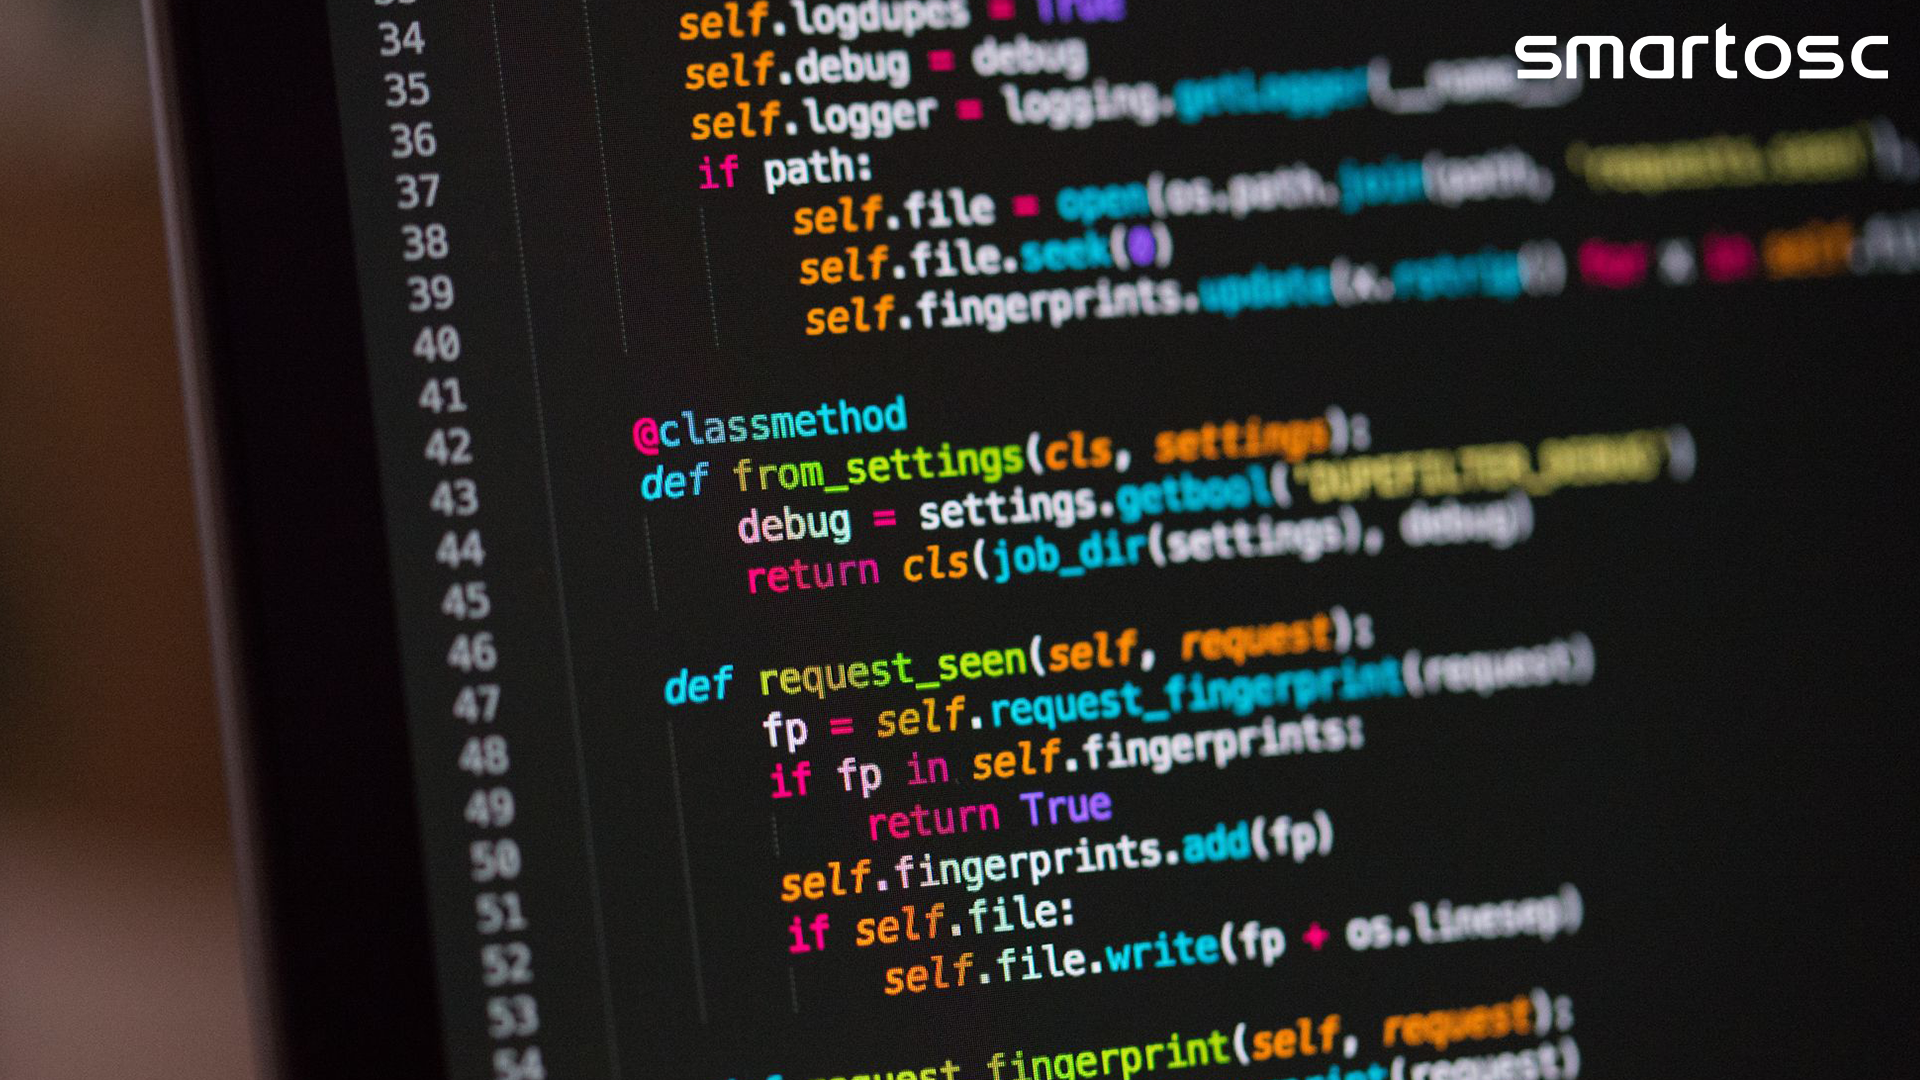
\includegraphics[width=14cm]{Python2.png}\\
Applications of Python
\end{center}
\end{figure}



\textbf{7. Financial and Trading Applications:}
\begin{itemize}
    \item In the financial industry, Python is used for quantitative analysis, algorithmic trading, and financial modeling. Libraries like QuantLib and Zipline help in building trading systems and performing risk analysis.
\end{itemize}

\textbf{8. Game Development:}
\begin{itemize}
    \item Python can be used for game development with libraries like Pygame, which provides functionality for developing simple 2D games and multimedia applications.
\end{itemize}

\textbf{9. Education:}
\begin{itemize}
    \item Python’s simplicity makes it an excellent language for teaching programming and computer science concepts to beginners. It is widely used in academic courses and coding bootcamps.
\end{itemize}

\textbf{10. Internet of Things (IoT):}
\begin{itemize}
    \item Python can run on microcontrollers and single-board computers like Raspberry Pi, making it suitable for IoT projects. Libraries like MicroPython and CircuitPython extend its functionality in this domain.
\end{itemize}

\textbf{11. Cybersecurity:}
\begin{itemize}
    \item Python is used in cybersecurity for tasks such as penetration testing, network scanning, and developing security tools. Libraries like Scapy and frameworks like PyCrypto are commonly used.
\end{itemize}

\textbf{12. Bioinformatics:}
\begin{itemize}
    \item In bioinformatics, Python is used for processing biological data, such as DNA sequencing. Libraries like Biopython provide tools for computational biology and bioinformatics research.
\end{itemize}


\subsection{Python’s distinctive features}
Python is considered a popular programming language in the programming community for its distinctive features such as:
\begin{itemize}
    \item It is an interpreted language, processed at runtime by the Python interpreter.
    \item It supports object-oriented programming features and techniques as an object-oriented programming language.
    \item It allows users to interact directly with the Python interpreter to write programs as an interactive programming language.
    \item It is very easy to learn, especially for beginners.
    \item Python syntax is easy to understand and not complicated, which also makes it popular.
    \item Python source code is clearly defined and can be easily observed by eye.
    \item Python code can run on multiple hardware platforms and is compatible with the same interface.
    \item Users can add low-level modules to the Python interpreter to extend the complexity of the program.
    \item Python provides an improved structure to support large programs after shell scripts.
\end{itemize}

\subsection{Popularity of Python}
Python's widespread popularity can be attributed to several key factors that make it an attractive choice for programmers across various domains. Here are some of the primary reasons for its popularity:

\begin{itemize}
    \item Python has a simple syntax that mimics natural language, making it easier to read and understand. This helps users develop and improve projects faster.
    \item Python is versatile and can be used for a variety of different tasks, from web development to machine learning.
    \item Python is beginner-friendly, making it a popular programming language for new programmers.
    \item Python is open source, so it is free and available for commercial purposes.
    \item Python’s repository of modules and libraries is vast and growing. These are code packages created by third-party users to extend the capabilities of Python.
    \item Python has a large and active community contributing to its repository of modules and libraries. This benefits other programmers when they need to find solutions to specific problems.
\end{itemize}

\begin{figure}[h!]
\begin{center}
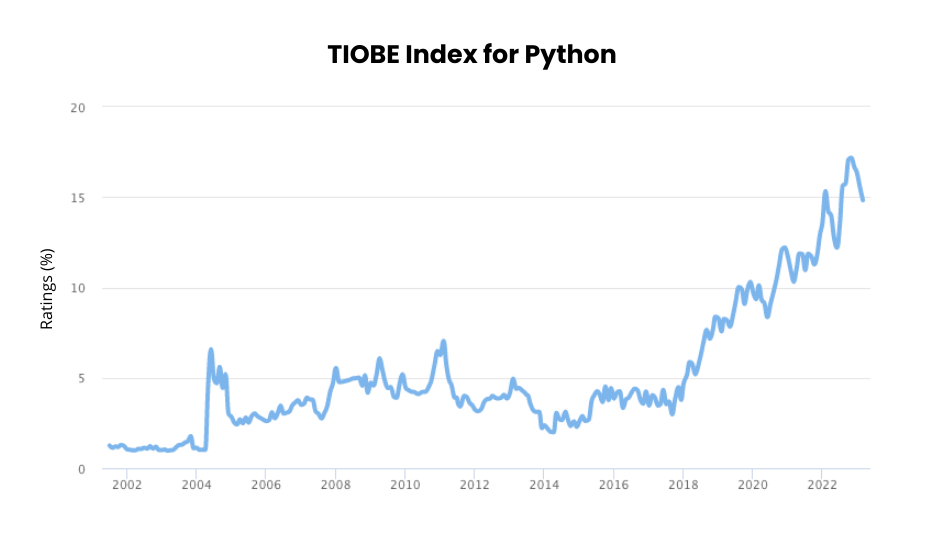
\includegraphics[width=11.5cm]{Python3.png}\\
Chart illustrate the popularity of Python
\end{center}
\end{figure}

\subsection{Strengths of Python}
Python has simple and easy-to-understand syntax, making it a suitable programming language for developers with limited experience and attracting a large community of users. Because there are many academics and professors in the community, when developers encounter problems, they can get quick support and don’t have to worry about the complexity of the language.

Python is developed under an open source license approved by OSI, so it is a free language to use and distribute, including for commercial purposes. This helps reduce maintenance costs and developers can share, copy, and customize it. For the Python community, this is an opportunity to share knowledge and experience with newcomers.

Python is said to be very easy to use. Although when developing mobile applications or games, there may be other languages such as C++ or other scripting languages that are easier to use, but Python still gives better results in building server-side applications, automating system building processes, and collecting test data.

Python has many libraries and frameworks to choose from, which is one of the great advantages of Python. From NumPy to TensorFlow, Python libraries are used for everything from data visualization, machine learning, data science, natural language processing, and complex data analysis.

Python has a large library that supports memory management and has a bright design to increase productivity for Python programmers. Thanks to this, they can manage databases, documentation, web browsers, perform unit testing, and many other functions. In addition, Python can be used to develop web applications, desktop applications, complex computing systems, life support management systems, the Internet of Things (IoT), games, and more.

\section{Mechanism of Python}
\subsection{Python Execution Model}

\textbf{1. Python as an Interpreted Language}
\begin{itemize}
    \item \textbf{Interpreted Language:} Python is often referred to as an interpreted language, meaning that its code is executed line by line by an interpreter rather than being compiled into machine code beforehand.
    \item \textbf{Python Interpreter:} The most commonly used Python interpreter is CPython, which is written in C and is the reference implementation of Python.
\end{itemize}


\textbf{2. Compilation to Bytecode}
\begin{itemize}
    \item \textbf{Source Code:} When you write Python code, you create source code files with the .py extension.
    \item \textbf{Bytecode Compilation:} Before execution, Python code is compiled into bytecode. Bytecode is a low-level representation of your source code, which is platform-independent. This bytecode is stored in .pyc files located in the \_\_pycache\_\_ directory.

    \item \textbf{Intermediate Step:} This bytecode is an intermediate step between the source code and machine code. It is not human-readable but is more abstract than machine code.
\end{itemize}

\textbf{3. Execution in the Python Virtual Machine (PVM)}
\begin{itemize}
    \item \textbf{PVM:} The Python Virtual Machine (PVM) is the runtime engine that executes the compiled bytecode. It interprets the bytecode instructions and performs the corresponding operations on the machine.
    \item \textbf{Execution Process:} The PVM reads the bytecode instructions one by one and converts them to machine code that the underlying hardware can execute.
\end{itemize}

\begin{figure}[h!]
\begin{center}
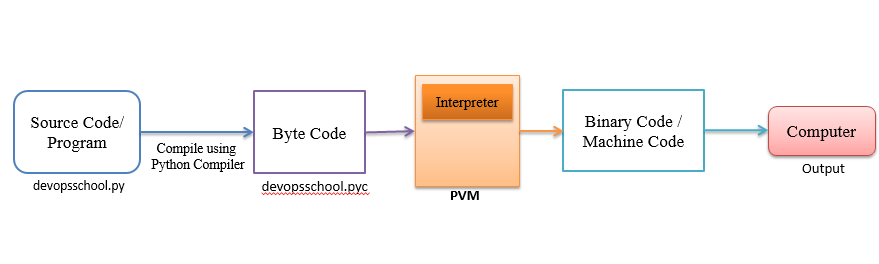
\includegraphics[width=12.5cm]{mechanism1.png}\\
Python Virtual Machine
\end{center}
\end{figure}


\subsection{Components of the Python Execution Model}

\textbf{1. Interpreter}
\begin{itemize}
    \item \textbf{CPython:} The default and most widely used implementation of Python. It compiles Python code into bytecode and interprets it using the PVM.
    \item \textbf{Other Implementations:} There are several other implementations of Python:\\
    + \textbf{PyPy:} An alternative implementation with a Just-In-Time (JIT) compiler that can significantly speed up the execution of Python code by compiling bytecode to machine code at runtime.\\
    + \textbf{Jython:} An implementation of Python that runs on the Java platform.\\
    + \textbf{IronPython:} AAn implementation of Python for the .NET framework.\\
    + \textbf{MicroPython:} A lean implementation of Python for microcontrollers.\\
    
\end{itemize}

\textbf{2. Garbage Collection}
\begin{itemize}
    \item \textbf{Memory Management:} Python uses automatic memory management and garbage collection to reclaim memory occupied by objects that are no longer in use.
    \item \textbf{Reference Counting:} The primary mechanism for garbage collection in CPython is reference counting. Each object has a reference count, and when this count drops to zero, the memory occupied by the object is deallocated.
    \item \textbf{Cyclic Garbage Collector:} Python also has a cyclic garbage collector to detect and collect objects involved in reference cycles (objects referencing each other).
\end{itemize}

\begin{figure}[h!]
\begin{center}
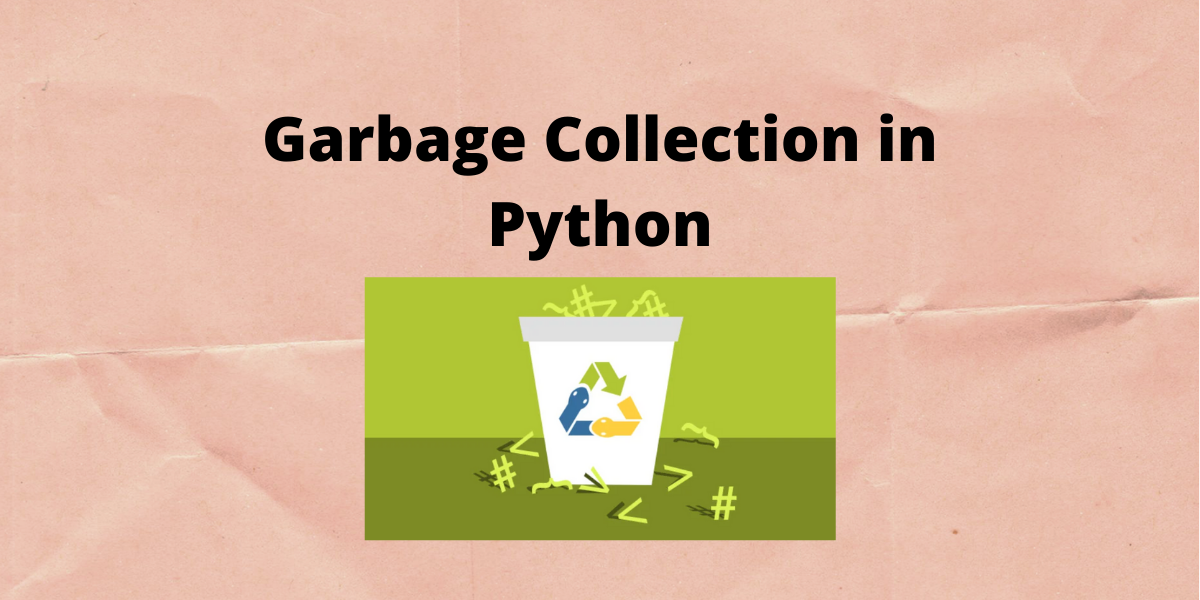
\includegraphics[width=12.5cm]{mechanism2.png}\\
Garbage Collection in Python
\end{center}
\end{figure}


\subsection{Just-In-Time (JIT) Compilation}

\textbf{PyPy's JIT Compiler:} PyPy includes a JIT compiler that translates Python bytecode into machine code at runtime, offering significant performance improvements for long-running programs.
\begin{itemize}
    \item \textbf{JIT Compilation:} Instead of interpreting bytecode every time it runs, the JIT compiler compiles frequently executed bytecode into machine code, which can be executed directly by the CPU.
    \item \textbf{Performance Benefits:} This approach can dramatically increase the execution speed of Python programs, especially for computationally intensive tasks.
\end{itemize}

\subsection{Python's Global Interpreter Lock (GIL)}
\textbf{1. Concurrency Limitation:} CPython uses a mechanism called the Global Interpreter Lock (GIL) to ensure that only one thread executes Python bytecode at a time. This simplifies memory management but limits the performance of multi-threaded programs.\\

\textbf{2. Workarounds:} To bypass the GIL and achieve true parallelism, you can use multiprocessing, which involves running multiple processes with separate memory spaces, or switch to implementations like Jython or IronPython, which do not have a GIL.\\

\subsection{Advanced Python Execution Insights}
\textbf{1. Abstract Syntax Trees (AST)}
\begin{itemize}
    \item \textbf{Parsing:} Before bytecode compilation, Python code is parsed into an Abstract Syntax Tree (AST), a tree representation of the source code's syntactic structure.
    \item \textbf{AST Module:} Python provides the `ast` module to interact with and manipulate the AST, allowing for advanced code analysis and transformation.
\end{itemize}


\textbf{2. Code Objects}
\begin{itemize}
    \item \textbf{Code Objects:} Python's `compile()`  function can compile source code into code objects, which can be executed by the `exec()` function.
\end{itemize}

\subsection{Summary}
Understanding Python's execution model involves knowing how it transitions from source code to execution through stages like parsing, bytecode compilation, and interpretation by the PVM. Advanced topics like JIT compilation, garbage collection, and handling the GIL offer deeper insights into Python's performance and concurrency mechanisms. This knowledge is crucial for optimizing Python code and leveraging different implementations for specific use cases.

\section{Advanced knowledge about python}

\subsection{Metaprogramming}
\textbf{Metaclasses:}
\begin{itemize}
    \item A metaclass in Python is a class of a class that defines how a class behaves. A class is an instance of a metaclass.
    \item Example of a metaclass:\\
    \begin{lstlisting}[language = Python]
    class Meta(type):
    def __new__(cls, name, bases, dct):
        print(f"Creating class {name}")
        return super().__new__(cls, name, bases, dct)
        
    class MyClass(metaclass=Meta):
        pass
    \end{lstlisting}
    
\end{itemize}

\textbf{Decorators:}
\begin{itemize}
    \item Functions or classes that modify the behavior of other functions or classes.
    \item Function decorator example:\\
    \begin{lstlisting}[language = Python]
    def decorator(func):
    def wrapper(*args, **kwargs):
        print("Something is happening before the function is called.")
        result = func(*args, **kwargs)
        print("Something is happening after the function is called.")
        return result
    return wrapper

    @decorator
    def say_hello():
        print("Hello!")
    \end{lstlisting}
    
\end{itemize}

\subsection{Concurrency and Parallelism}

\textbf{Threading:}
\begin{itemize}
    \item The `threading` module provides a way to run multiple threads (smaller units of a process) concurrently.
    \item Example:\\
    \begin{lstlisting}[language = Python]
    import threading

    def print_numbers():
        for i in range(10):
            print(i)
    
    thread = threading.Thread(target=print_numbers)
    thread.start()
    thread.join()
    \end{lstlisting}
    
\end{itemize}

\begin{figure}[h!]
\begin{center}
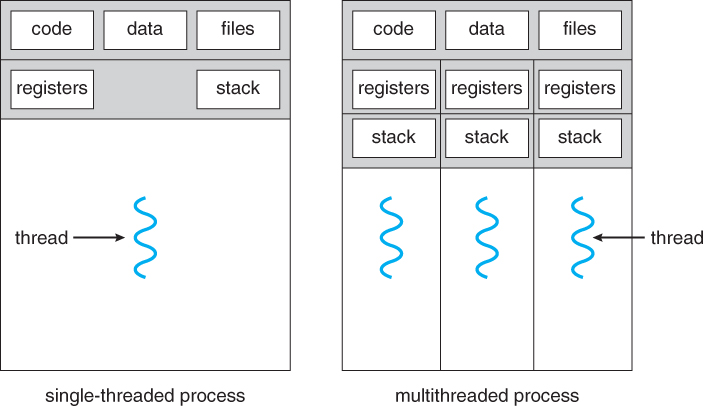
\includegraphics[width=10.5cm]{advanced1.jpg}\\
Threading of Python
\end{center}
\end{figure}


\textbf{Multiprocessing:}
\begin{itemize}
    \item The `multiprocessing` module allows you to create processes that run in parallel on different cores.
    \item Example:\\
    \begin{lstlisting}[language = Python]
    from multiprocessing import Process

    def print_numbers():
        for i in range(10):
            print(i)
    
    process = Process(target=print_numbers)
    process.start()
    process.join()
    \end{lstlisting}
    
\end{itemize}

\begin{figure}[h!]
\begin{center}
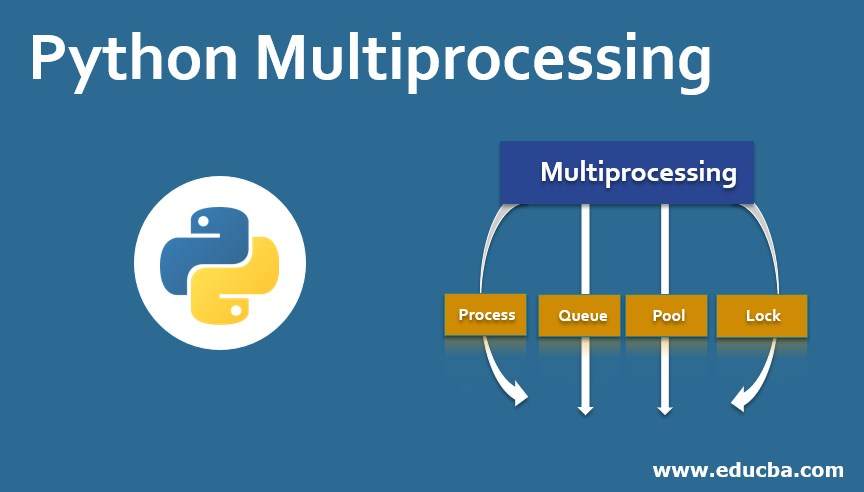
\includegraphics[width=12.5cm]{advanced2.jpg}\\
Multiprocessor of Python
\end{center}
\end{figure}


\textbf{Asyncio:}
\begin{itemize}
    \item The `asyncio` library provides support for asynchronous programming, enabling you to write concurrent code using the `async`/`await` syntax.

    \item Example:\\
    \begin{lstlisting}[language = Python]
    import asyncio

    async def say_hello():
        await asyncio.sleep(1)
        print("Hello!")
    
    async def main():
        await say_hello()
    
    asyncio.run(main())
    \end{lstlisting}
    
\end{itemize}

\begin{figure}[h!]
\begin{center}
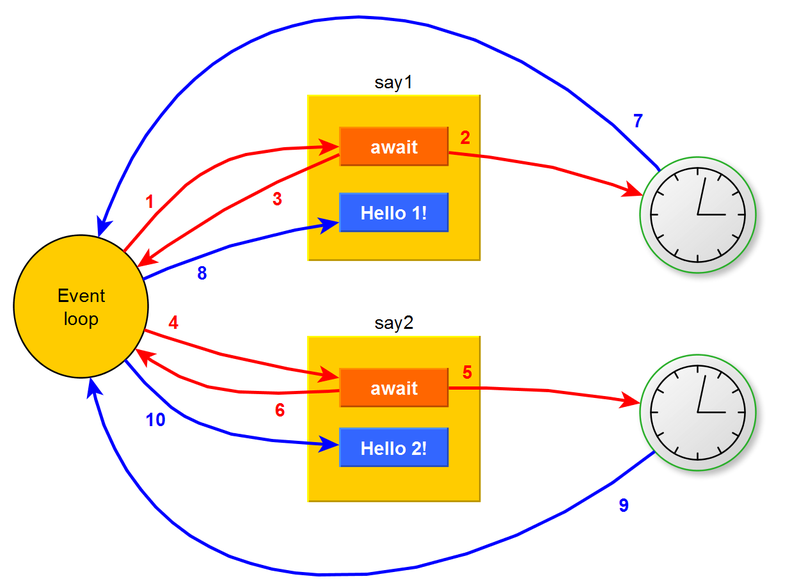
\includegraphics[width=12.5cm]{advanced3.png}\\
Asyncio of Python
\end{center}
\end{figure}


\subsection{Advanced Data Structures}

\textbf{Deque:}
\begin{itemize}
    \item A double-ended queue, `collections.deque`, supports fast appends and pops from both ends.

    \item Example:\\
    \begin{lstlisting}[language = Python]
    from collections import deque

    d = deque()
    d.append(1)
    d.appendleft(2)
    print(d)  # deque([2, 1])
    \end{lstlisting}
    
\end{itemize}

\textbf{Namedtuple:}
\begin{itemize}
    \item Immutable, lightweight objects that can be used in place of tuples and dictionaries.

    \item Example:\\
    \begin{lstlisting}[language = Python]
    from collections import namedtuple

    Point = namedtuple('Point', ['x', 'y'])
    p = Point(1, 2)
    print(p.x, p.y)  # 1 2
    \end{lstlisting}
    
\end{itemize}


\begin{figure}[h!]
\begin{center}
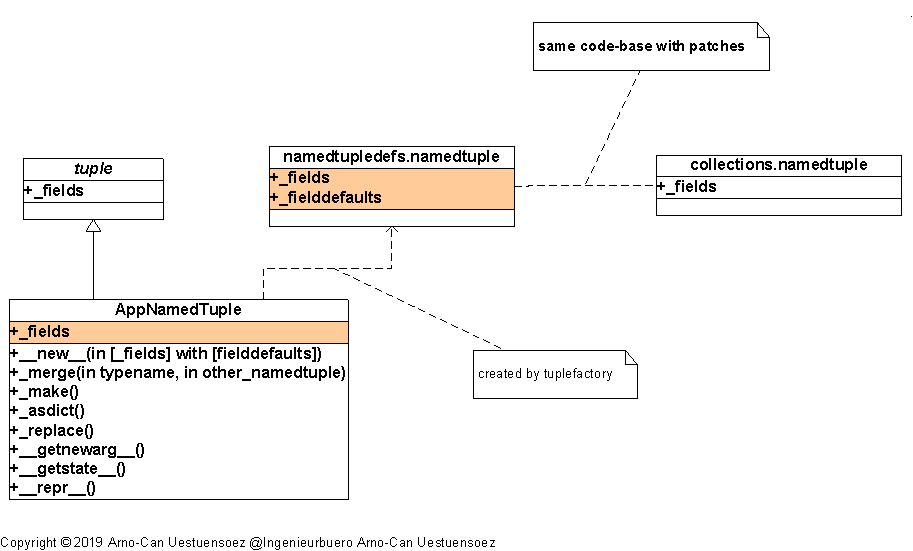
\includegraphics[width=12.5cm]{advanced4.png}\\
Namedtuple of Python
\end{center}
\end{figure}



\subsection{Descriptors}

\textbf{Namedtuple:}
\begin{itemize}
    \item Descriptors manage the attributes of different classes using methods in a class.

    \item Example:\\
    \begin{lstlisting}[language = Python]
    class Descriptor:
    def __get__(self, instance, owner):
        return f"Value accessed from {instance}"

    class MyClass:
        attribute = Descriptor()
    
    obj = MyClass()
    print(obj.attribute)
    \end{lstlisting}
    
\end{itemize}

\subsection{Context Managers and the `with` Statement}

\textbf{Contextlib:}
\begin{itemize}
    \item The `contextlib` module provides utilities for working with context managers.

    \item Example:\\
    \begin{lstlisting}[language = Python]
    from contextlib import contextmanager

    @contextmanager
    def open_file(name):
        f = open(name, 'w')
        try:
            yield f
        finally:
            f.close()
    
    with open_file('test.txt') as f:
        f.write('Hello, world!')
    \end{lstlisting}
    
\end{itemize}

\begin{figure}[h!]
\begin{center}

\includegraphics[width=10.5cm]{advanced5.jpg}\\
Contextlib of Python
\end{center}
\end{figure}


\subsection{Testing}

\textbf{Unittest:}
\begin{itemize}
    \item Python's built-in library for testing.

    \item Example:\\
    \begin{lstlisting}[language = Python]
    import unittest

    def add(a, b):
        return a + b
    
    class TestAdd(unittest.TestCase):
        def test_add(self):
            self.assertEqual(add(1, 2), 3)
    
    if __name__ == '__main__':
        unittest.main()
    \end{lstlisting}
    
\end{itemize}

\begin{figure}[h!]
\begin{center}

\includegraphics[width=12.5cm]{advanced6.jpg}\\
Unittest in Python
\end{center}
\end{figure}

\textbf{Pytest:}
\begin{itemize}
    \item A popular third-party testing framework.

    \item Example:\\
    \begin{lstlisting}[language = Python]
    def add(a, b):
    return a + b

    def test_add():
        assert add(1, 2) == 3
    \end{lstlisting}
    
\end{itemize}

\subsection{Memory Management}

\textbf{Garbage Collection:}
\begin{itemize}
    \item Python uses automatic garbage collection for memory management.

    \item Example:\\
    \begin{lstlisting}[language = Python]
    import gc

    gc.collect()
    \end{lstlisting}
    
\end{itemize}


\textbf{Weak References:}
\begin{itemize}
    \item Manage references to objects without preventing their garbage collection using `weakref`.

    \item Example:\\
    \begin{lstlisting}[language = Python]
    import weakref

    class MyClass:
        pass
    
    obj = MyClass()
    r = weakref.ref(obj)
    print(r())
    del obj
    print(r())
    \end{lstlisting}
    
\end{itemize}

\subsection{C Extensions}

\textbf{Cython:}
\begin{itemize}
    \item A superset of Python designed to give C-like performance.

    \item Example:\\
    \begin{lstlisting}[language = Python]
    cpdef int add(int a, int b):
    return a + b
    \end{lstlisting}
    
\end{itemize}

\begin{figure}[h!]
\begin{center}
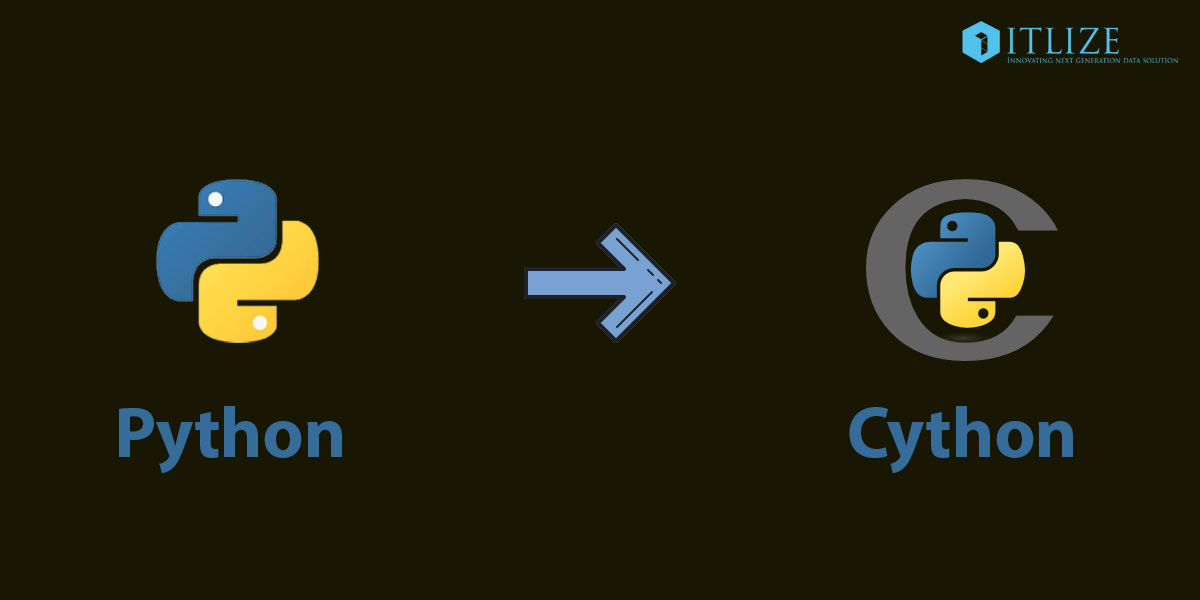
\includegraphics[width=10.5cm]{advanced7.jpg}\\
Python to Cython
\end{center}
\end{figure}



\textbf{ctypes:}
\begin{itemize}
    \item Allows calling functions in DLLs or shared libraries.

    \item Example:\\
    \begin{lstlisting}[language = Python]
    from ctypes import CDLL

    libc = CDLL('libc.so.6')
    libc.printf(b"Hello, world!\n")
    \end{lstlisting}
    
\end{itemize}

\subsection{Networking}

\textbf{Sockets:}
\begin{itemize}
    \item Low-level network interface.

    \item Example:\\
    \begin{lstlisting}[language = Python]
    import socket

    s = socket.socket(socket.AF_INET, socket.SOCK_STREAM)
    s.connect(('www.python.org', 80))
    s.sendall(b'GET / HTTP/1.1\r\nHost: www.python.org\r\n\r\n')
    data = s.recv(1024)
    s.close()
    print(data)
    \end{lstlisting}
    
\end{itemize}

\begin{figure}[h!]
\begin{center}
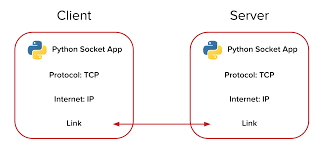
\includegraphics[width=10.5cm]{advanced8.png}\\
Sockets illustration in Python
\end{center}
\end{figure}


\textbf{Asyncio Networking:}
\begin{itemize}
    \item High-level asynchronous networking with `asyncio`.

    \item Example:\\
    \begin{lstlisting}[language = Python]
    import asyncio

    async def handle_echo(reader, writer):
        data = await reader.read(100)
        writer.write(data)
        await writer.drain()
        writer.close()
    
    async def main():
        server = await asyncio.start_server(handle_echo, '127.0.0.1', 8888)
        async with server:
            await server.serve_forever()
    
    asyncio.run(main())
    \end{lstlisting}
    
\end{itemize}


\subsection{Advanced Libraries and Tools}

\textbf{Pandas:}
\begin{itemize}
    \item Data analysis library.

    \item Example:\\
    \begin{lstlisting}[language = Python]
    import pandas as pd

    df = pd.DataFrame({
        'A': [1, 2, 3],
        'B': [4, 5, 6]
    })
    print(df)
    \end{lstlisting}
    
\end{itemize}

% \begin{figure}[h!]
% \begin{center}
% 
\includegraphics[width=10.5cm]{advanced9.png}\\
% Pandas in Python
% \end{center}
% \end{figure}



\textbf{NumPy:}
\begin{itemize}
    \item Library for numerical computations.

    \item Example:\\
    \begin{lstlisting}[language = Python]
    import numpy as np

    arr = np.array([1, 2, 3])
    print(arr * 2)
    \end{lstlisting}
    
\end{itemize}

\textbf{Scikit-learn:}
\begin{itemize}
    \item Machine learning library.

    \item Example:\\
    \begin{lstlisting}[language = Python]
    from sklearn.linear_model import LinearRegression
    import numpy as np
    
    X = np.array([[1, 1], [1, 2], [2, 2], [2, 3]])
    y = np.dot(X, np.array([1, 2])) + 3
    
    reg = LinearRegression().fit(X, y)
    print(reg.coef_)
    \end{lstlisting}
    
\end{itemize}


\section{Characteristic of python about functional programming }
Python is a multi-paradigm language that supports functional programming, among other paradigms. Here are the key characteristics of Python related to functional programming:

\textbf{1. First-Class Functions:} In Python, functions are first-class objects, meaning they can be assigned to variables, passed as arguments, and returned from other functions. This allows for higher-order functions, which can accept other functions as arguments and return them as well.
\begin{lstlisting}[language = Python]
def add(x, y):
    return x + y

def apply_function(f, x, y):
    return f(x, y)

result = apply_function(add, 5, 3)
print(result)  # Output: 8
\end{lstlisting}

\vspace{0.5cm}

\textbf{2. Anonymous Functions (Lambdas):} Python supports anonymous functions, also known as lambda functions, which are small, unnamed functions defined using the lambda keyword. They are often used for short, throwaway functions.
\begin{lstlisting}[language = Python]
add = lambda x, y: x + y
print(add(5, 3))  # Output: 8
\end{lstlisting}

\vspace{0.5cm}

\textbf{3. Higher-Order Functions:} Python allows the creation of higher-order functions, which are functions that operate on other functions by taking them as arguments or returning them.
\begin{lstlisting}[language = Python]
def increment(x):
    return x + 1

def apply_twice(f, x):
    return f(f(x))

result = apply_twice(increment, 3)
print(result)  # Output: 5
\end{lstlisting}

\vspace{0.5cm}

\textbf{4. Immutability:} Functional programming emphasizes immutability, where data cannot be modified after it is created. While Python does not enforce immutability, it provides immutable data structures like tuples and frozensets, and encourages the use of immutable types where appropriate.
\begin{lstlisting}[language = Python]
a = (1, 2, 3)
# a[0] = 4  # This would raise a TypeError
\end{lstlisting}

\vspace{0.5cm}

\textbf{5. Pure Functions:} Functional programming favors pure functions, which have no side effects and return the same output given the same inputs. Python allows for the creation of pure functions, which can make the code more predictable and easier to test.
\begin{lstlisting}[language = Python]
def pure_function(x, y):
    return x + y
\end{lstlisting}

\vspace{0.5cm}

\textbf{6. Recursion:} Functional programming often uses recursion as a primary means of iteration. Python supports recursion, though it has a recursion limit to prevent infinite recursion.
\begin{lstlisting}[language = Python]
def factorial(n):
    if n == 0:
        return 1
    else:
        return n * factorial(n - 1)

print(factorial(5))  # Output: 120
\end{lstlisting}

\vspace{0.5cm}

\textbf{7. Functional Tools in `functools`: } Python’s `functools` module provides higher-order functions and tools that support functional programming, such as `reduce`, `partial`, and `lru\_cache` and return them as well.
\begin{lstlisting}[language = Python]
from functools import reduce

numbers = [1, 2, 3, 4, 5]
product = reduce(lambda x, y: x * y, numbers)
print(product)  # Output: 120
\end{lstlisting}

\vspace{0.5cm}

\textbf{8. Comprehensions and Generator Expressions:} Python comprehensions (list, set, dictionary comprehensions) and generator expressions provide concise ways to construct new sequences and lazily evaluated iterators, often used in functional programming.
\begin{lstlisting}[language = Python]
squares = [x ** 2 for x in range(10)]
print(squares)  # Output: [0, 1, 4, 9, 16, 25, 36, 49, 64, 81]

gen = (x ** 2 for x in range(10))
for square in gen:
    print(square, end=" ")  # Output: 0 1 4 9 16 25 36 49 64 81
\end{lstlisting}

\vspace{0.5cm}

\textbf{9. Map, Filter, and Reduce:} Python includes built-in functions `map`, `filter`, and `reduce` (in the `functools` module) for functional-style processing of sequences.
\begin{lstlisting}[language = Python]
numbers = [1, 2, 3, 4, 5]
squares = map(lambda x: x ** 2, numbers)
evens = filter(lambda x: x % 2 == 0, numbers)

print(list(squares))  # Output: [1, 4, 9, 16, 25]
print(list(evens))    # Output: [2, 4]
\end{lstlisting}

\vspace{0.5cm}

\textbf{10. Decorators:} Python decorators provide a way to modify or enhance functions or methods without changing their actual code. They are a powerful feature often used in functional programming to apply higher-order functions.
\begin{lstlisting}[language = Python]
def decorator_function(original_function):
    def wrapper_function(*args, **kwargs):
        print("Wrapper executed this before {}".format(original_function.__name__))
        return original_function(*args, **kwargs)
    return wrapper_function

@decorator_function
def display():
    print("Display function ran")

display()
# Output:
# Wrapper executed this before display
# Display function ran
\end{lstlisting}

\vspace{0.5cm}

\section{Set Up a Virtual Environment in Python}
When developing software with Python, a basic approach involves installing Python on your machine, installing necessary libraries via the terminal, writing code in a single .py file or notebook, and running your Python program in the terminal. This method is common for beginners and those transitioning from using Python for data analytics.\\

While this approach works for simple scripting projects, more complex software development projects—like building a Python library, an API, or a software development kit—require working with multiple files, packages, and dependencies. This necessitates isolating the Python development environment for each project.\\

Consider this scenario: you are working on app A, using your system-installed Python, and you use `pip` to install packageX version 1.0 globally. Then you switch to project B and install packageX version 2.0, which has breaking changes from version 1.0. When you return to app A, you encounter errors because of these changes, and your app does not run. This issue can arise when building software with Python. To avoid it, you can use virtual environments.\\

This tutorial will explain everything you need to know about virtual environments and how to set one up with \textbf{Virtualenv}.\\

\subsection{Virtual Environment}

\textit{"A virtual environment is a Python environment such that the Python interpreter, libraries and scripts installed into it are isolated from those installed in other virtual environments, and (by default) any libraries installed in a “system” Python, i.e., one which is installed as part of your operating system"}\\

To break this down, when you activate a virtual environment for your project, your project becomes its own self contained application, independent of the system installed Python and its modules.\\

Your new virtual environment has its own pip to install libraries, its own libraries folder, where new libraries are added, and its own Python interpreter for the Python version you used to activate the environment.\\

With this new environment, your application becomes self-contained and you get some benefits such as:
\begin{itemize}
    \item Your development environment is contained within your project, becomes isolated, and does not interfere with your system installed Python or other virtual environments
    \item You can create a new virtual environment for multiple Python versions
    \item You are able to download packages into your project without admin privileges
    \item You can easily package your application and share with other developers to replicate
    \item You can easily create a list of dependencies and sub dependencies in a file, for your project, which makes it easy for other developers to replicate and install all the dependencies used within your environment
\end{itemize}
Using virtual environments is recommended for software development projects that generally grow out of a single Python script, and Python provides multiple ways of creating and using a virtual environment.\\

In the sections below, we will walk through how to set up your virtual environment, using \textbf{venv}, which gives you a lot more low level control of your environment.\\

Another common way to set up your virtual environment is to use \textbf{pipenv}, which is a more high level approach.\\

\subsection{Install a Virtual Environment using Venv}
\textbf{Virtualenv} is a tool to set up your Python environments. Since Python 3.3, a subset of it has been integrated into the standard library under the venv module. You can install venv to your host Python by running this command in your terminal:\\
\begin{lstlisting}[language = ]
    pip install virtualenv
\end{lstlisting}


To use venv in your project, in your terminal, create a new project folder, cd to the project folder in your terminal, and run the following command:
\begin{lstlisting}[language = ]
    python<version> -m venv <virtual-environment-name>
\end{lstlisting}

Like so:

\begin{lstlisting}[language = ]
    mkdir projectA
    cd projectA
    python3.8 -m venv env
\end{lstlisting}

When you check the new projectA folder, you will notice that a new folder called env has been created. \textbf{env} is the name of our virtual environment, but it can be named anything you want.\\

If we check the contents of env for a bit, on a Mac you will see a bin folder. You will also see scripts that are typically used to control your virtual environment, such as activate and pip to install libraries, and the Python interpreter for the Python version you installed, and so on. (This folder will be called Scripts on windows).\\

The lib folder will contain a list of libraries that you have installed. If you take a look at it, you will see a list of the libraries that come by default with the virtual environment.\\

\subsection{Conclusion}

% Python virtual environments are an essential tool for developers, offering the ability to create isolated environments for individual projects. This isolation means that each project can have its own dependencies, libraries, and even Python versions, separate from the system-wide Python installation and other projects. By using virtual environments, you gain full control over the project's setup, ensuring that your development process is both clean and organized.\\

One of the key benefits of virtual environments is that they help maintain consistent development conditions across different machines and team members. When you share your project with others or deploy it to a production environment, the virtual environment ensures that all required packages and versions are identical to those you used during development. This reproducibility eliminates the common "it works on my machine" problem and makes it easier to debug and manage applications.\\

For developers transitioning from writing simple .py scripts or working within Jupyter notebooks to building more complex applications, incorporating virtual environments is a crucial step. It helps manage dependencies more effectively and avoids conflicts that can arise when multiple projects require different versions of the same package. Furthermore, virtual environments can help prevent unintentional modifications to the system Python installation, which can affect other applications and lead to difficult-to-trace bugs.\\

Setting up and using a virtual environment is straightforward and brings numerous benefits to your development workflow. By creating an isolated space for each project, you ensure that your project environment remains consistent and manageable, from development through to deployment. Now that you understand the advantages and know how to set up a virtual environment, you can enhance your development process and ensure your projects are well-organized and easily reproducible.\\

\section{How to create a functional program in Python}
Creating a functional program in Python involves leveraging the principles of functional programming (FP), such as immutability, first-class functions, higher-order functions, and pure functions. Here's a step-by-step guide to help you create a functional program in Python:

\subsection{Step 1: Understand Functional Programming Principles}
\textbf{1. Immutability:} Avoid changing state or mutable data.
\textbf{2. Pure Functions:} Functions should return the same result for the same inputs and have no side effects.
\textbf{3. First-Class Functions:} Treat functions as first-class citizens. You can pass them as arguments, return them from other functions, and assign them to variables.
\textbf{4. Higher-Order Functions:} Functions that take other functions as arguments or return them as results.

\subsection{Step 2: Set Up Your Python Environment}

Ensure you have Python installed on your system. You can check your installation by running:
\begin{lstlisting}[language = sh]
    python --version
\end{lstlisting}

\subsection{Step 3: Write Functional Code}

\textbf{- Define Pure Functions}

Define pure functions that perform operations without side effects.
\begin{lstlisting}[language = Python]
    # Pure function to double a number
    def double(x):
        return x * 2
    
    # Pure function to check if a number is even
    def is_even(x):
        return x % 2 == 0
\end{lstlisting}

\textbf{- Use Higher-Order Functions}
Use built-in higher-order functions like `map`, `filter`, and `reduce`.

\begin{lstlisting}[language = Python]
    from functools import reduce

    # List of numbers
    numbers = [1, 2, 3, 4, 5, 6, 7, 8, 9, 10]
    
    # Map: Apply the double function to each element
    doubled_numbers = list(map(double, numbers))
    print("Doubled Numbers:", doubled_numbers)
    
    # Filter: Filter out only even numbers
    even_numbers = list(filter(is_even, numbers))
    print("Even Numbers:", even_numbers)
    
    # Reduce: Sum all numbers
    sum_of_numbers = reduce(lambda x, y: x + y, numbers)
    print("Sum of Numbers:", sum_of_numbers)
\end{lstlisting}


\subsection{Step 4: Avoid Mutable State}

Avoid using variables that can change state. Instead, work with immutable data structures.
\begin{lstlisting}[language = Python]
    # Instead of mutating a list, use a new list
    def add_one_to_each(numbers):
        return [x + 1 for x in numbers]
    
    original_numbers = [1, 2, 3]
    new_numbers = add_one_to_each(original_numbers)
    print("Original Numbers:", original_numbers)
    print("New Numbers:", new_numbers)
\end{lstlisting}

\subsection{Step 5: Compose Functions}
Compose small functions to build more complex functionality.
\begin{lstlisting}[language = Python]
    # Composing functions: Double the numbers and then filter out even numbers
    def double_and_filter_even(numbers):
        return list(filter(is_even, map(double, numbers)))
    
    composed_result = double_and_filter_even(numbers)
    print("Doubled and Filtered Even Numbers:", composed_result)
\end{lstlisting}
\subsection{Step 6: Test Your Functional Program}

To ensure your functions perform correctly, it's essential to write comprehensive tests using Python's `unittest` module or third-party libraries like `pytest`. Begin by importing the testing framework and defining a test case class that inherits from `unittest.TestCase`. Within this class, write methods that test specific aspects of your functions, using assert methods such as `assertEqual` to verify that the outputs match expected results. For instance, to test a simple `add` function, you might include methods to check the addition of positive numbers, negative numbers, and zero. Finally, run your tests by executing `unittest.main()` if the script is run directly, which will execute all test methods and report any failures, ensuring your code works as intended.

\section{Write a demo}
Let's develop a simple Formula 1 racing game that showcases the characteristics of functional programming. In functional programming, we emphasize the use of pure functions, immutability, and higher-order functions, avoiding mutable state and side effects. In our racing game, we'll design the core logic using pure functions to calculate positions, velocities, and lap times based on the current state of the race and the input from the player. By maintaining immutability, we'll ensure that each update to the game state results in a new state rather than modifying the existing one. Higher-order functions will enable us to abstract common patterns and operations, making our code more modular and reusable. Additionally, we'll use functional concepts like map, filter, and reduce to process collections of data efficiently. This approach will not only make our codebase cleaner and more maintainable but also enhance the reliability and predictability of the game by minimizing unexpected side effects and bugs. Through this example, we aim to demonstrate how functional programming principles can be effectively applied to game development, leading to a robust and scalable application.

\begin{figure}[h!]
\begin{center}
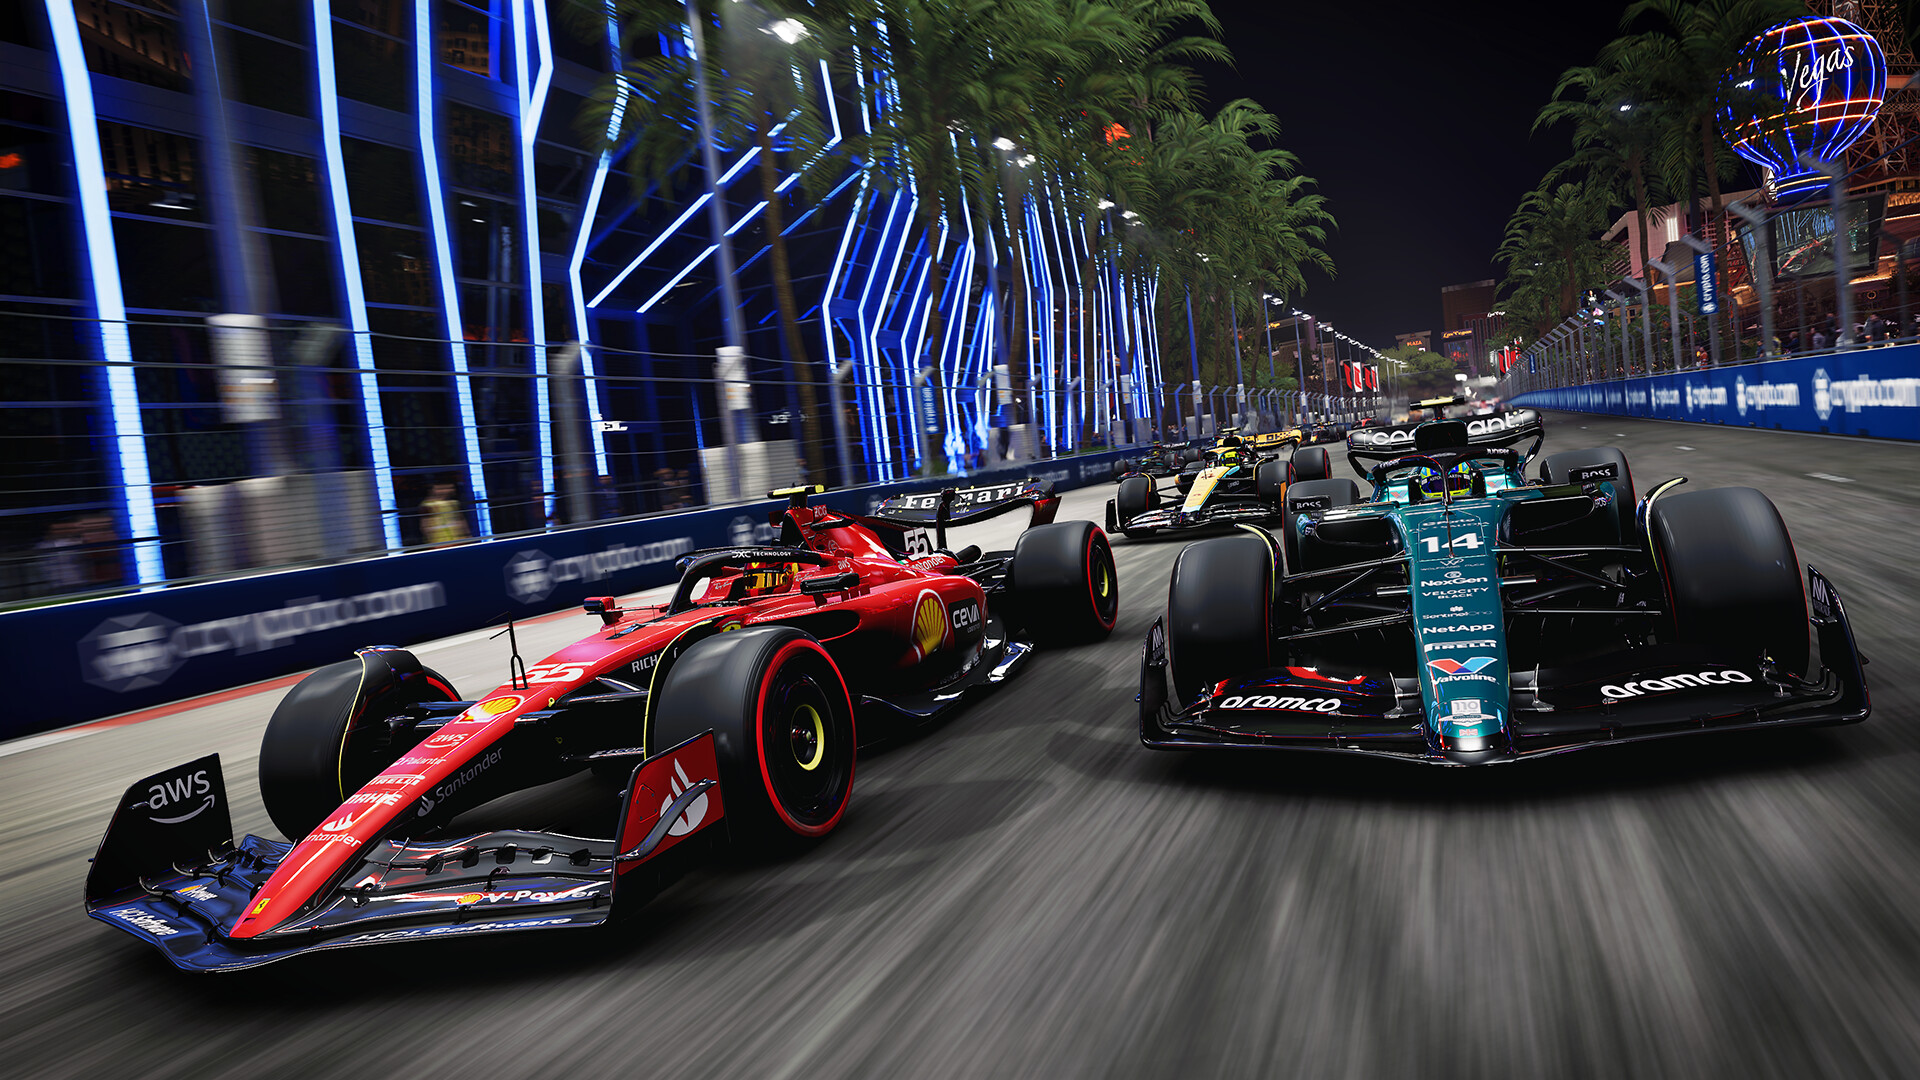
\includegraphics[width=10.5cm]{demo1.jpg}\\
Formula 1 Grand Prix Racing
\end{center}
\end{figure}

\subsection{Demo Code}

\begin{lstlisting}[language = Python]
    import random
    from typing import Tuple, Callable
    
    # Define track segments
    track_segments = ["straight", "turn", "straight", "turn", "straight", "finish"]
    
    # Functional approach to get player's speed choice
    def get_player_speed() -> int:
        while True:
            try:
                speed = int(input("Choose your speed (1-3): "))
                if speed in [1, 2, 3]:
                    return speed
                else:
                    print("Invalid speed. Please choose a speed between 1 and 3.")
            except ValueError:
                print("Invalid speed. Please choose a speed between 1 and 3.")
    
    # Functional approach to simulate car movement
    def move_car(position: int, speed: int, segment: str) -> int:
        if segment == "turn" and (speed == 3 or speed == 2):
            print("You crashed on a turn!")
            return 0  # crash
        return position + speed
    
    # Functional approach to simulate a single segment
    def play_segment(position: int, segment: str) -> Tuple[int, bool]:
        print(f"Current segment: {segment}")
        speed = get_player_speed()
        new_position = move_car(position, speed, segment)
        if new_position == 0:
            return position, True  # crashed
        print(f"New position: {new_position}\n")
        return new_position, False  # not crashed
    
    # Main function to play the game
    def main() -> None:
        print("Welcome to the Formula 1 Racing Game!")
        position = 0
        crashed = False
    
        for segment in track_segments:
            position, crashed = play_segment(position, segment)
            if crashed:
                print("Game Over! You crashed.")
                break
            if segment == "finish":
                break
        if not crashed:
            if position < len(track_segments) * 2:
                    print("Game Over! You did not reach the finish line in time.")
            else: 
                    print("Congratulations! You reached the finish line.")
    
    if __name__ == "__main__":
        main()
\end{lstlisting}


\textit{\textbf{Track Segments}}
\begin{description}
    \item[Definition:] A list that represents the different parts of the track.
    \item[Types]:
    \begin{description}
        \item[Straight:] A segment where the car can move safely at any speed.
        \item[Turn:] A segment where the car has a risk of crashing if moving too fast.
        \item[Finish Line:] The final segment indicating the end of the race.
    \end{description}
\end{description}

\textit{\textbf{get\_player\_speed}}
\begin{description}
    \item[Purpose:] To prompt the player to choose a speed for the current segment.
    \item[Speed Options]:
    \begin{description}
        \item[1:] Slow speed, safe for all segments.
        \item[2:] Medium speed, safe for all segments.
        \item[3:] High speed, risky on turns.
    \end{description}
    \item[Input Validation]:
    \begin{itemize}
        \item Ensures the input is a number.
        \item Ensures the number is between 1 and 3.
        \item Re-prompts the player if the input is invalid.
    \end{itemize}
\end{description}

\textit{\textbf{move\_car}}
\begin{description}
    \item[Purpose:] To update the car's position based on the chosen speed and current segment type.
    \item[Parameters]:
    \begin{description}
        \item[position:] The current position of the car on the track.
        \item[speed:] The speed chosen by the player.
        \item[segment\_type:] The type of the current track segment.
    \end{description}
    \item[Logic]:
    \begin{itemize}
        \item If \textit{segment\_type} is a turn and \textit{speed} is 3, the car crashes.
        \item If the car crashes, the position is reset to the start (position 0).
        \item If the car does not crash, the position is updated based on the speed.
    \end{itemize}
\end{description}

\textit{\textbf{play\_segment}}
\begin{description}
    \item[Purpose:] To simulate a single segment of the race.
    \item[Process]:
    \begin{itemize}
        \item Get the player's speed choice using \textit{get\_player\_speed}.
        \item Update the car's position using \textit{move\_car}.
        \item Check for crashes:
        \begin{itemize}
            \item If the car crashed, end the segment with a crash notification.
            \item If the car did not crash, move to the next segment.
        \end{itemize}
    \end{itemize}
\end{description}

\textit{\textbf{main}}
\begin{description}
    \item[Purpose:] To initialize and run the game.
    \item[Steps]:
    \begin{enumerate}
        \item Initialize the car's starting position.
        \item Define the track segments.
        \item Iterate through each track segment:
        \begin{itemize}
            \item Use \textit{play\_segment} to simulate each segment.
            \item If the car reaches the finish line, declare the player a winner.
            \item If the car crashes, end the game with a crash notification.
        \end{itemize}
    \end{enumerate}
    \item[Game End Conditions]:
    \begin{description}
        \item[Victory:] The car successfully navigates all segments and reaches the finish line.
        \item[Crash:] The car crashes on a turn by going too fast.
    \end{description}
\end{description}

\textit{\textbf{Detailed Explanation}}
\begin{description}
    \item[Initialization:] The game starts with the car at position 0 and a predefined set of track segments.
    \item[Gameplay]:
    \begin{itemize}
        \item The player is prompted to choose a speed for each segment.
        \item The car's position is updated based on the chosen speed and the segment type.
        \item If the car crashes on a turn (choosing speed 3 on a turn), the game ends with a crash message.
        \item If the car reaches the finish line without crashing, the player wins.
    \end{itemize}
    \item[Input Handling]:
    \begin{itemize}
        \item Ensures that the player's input is valid and within the acceptable range.
        \item Provides feedback if the input is invalid and re-prompts the player.
    \end{itemize}
\end{description}


\subsection{Output of the game}
\subsubsection{When the car crash}
Whenever the car approaches a turn on the track and selects a speed greater than 1, it will inevitably crash. This rule adds a layer of strategic risk management to the game. The track is divided into different segments, with turns being particularly hazardous due to the difficulty of navigating sharp changes in direction at higher speeds. If the player chooses a speed of 2 or 3 when entering a turn, the game triggers an immediate crash, simulating the realistic challenge of maintaining control at high velocities. Consequently, players must carefully consider their speed, recognizing the need to slow down to a speed of 1 before turns to avoid crashing and resetting their progress to the starting point, thus emphasizing the importance of balancing speed and safety in the game.

\begin{figure}[h!]
\begin{center}
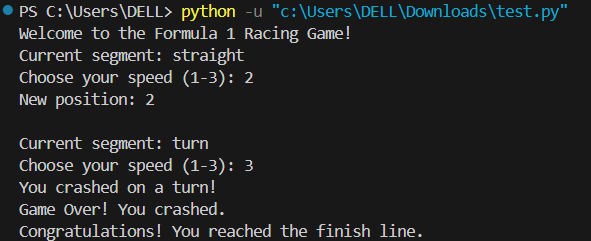
\includegraphics[width=10.5cm]{output1.png}\\
Output for the first scenario
\end{center}
\end{figure}

\subsubsection{Win the race}
When all the necessary conditions are met, and you successfully navigate the entire track, crossing the finish line without crashing or running out of time, you are crowned the champion of the Grand Prix Formula 1. Achieving this victory requires a careful balance of speed and strategy throughout the race. You must skillfully manage your car's speed, particularly when approaching turns, ensuring you slow down appropriately to avoid crashing. Successfully maintaining control of your car while maximizing your speed on straight segments will gradually advance you towards the finish line. Each segment you complete without incident brings you closer to the ultimate goal. Upon reaching the finish line, having skillfully maneuvered through every challenge and obstacle, your efforts are rewarded with the prestigious title of Grand Prix Formula 1 champion. This victory signifies not just the completion of the race but also the mastery of driving skills and strategic decision-making, culminating in a well-deserved triumph.

\begin{figure}[h!]
\begin{center}
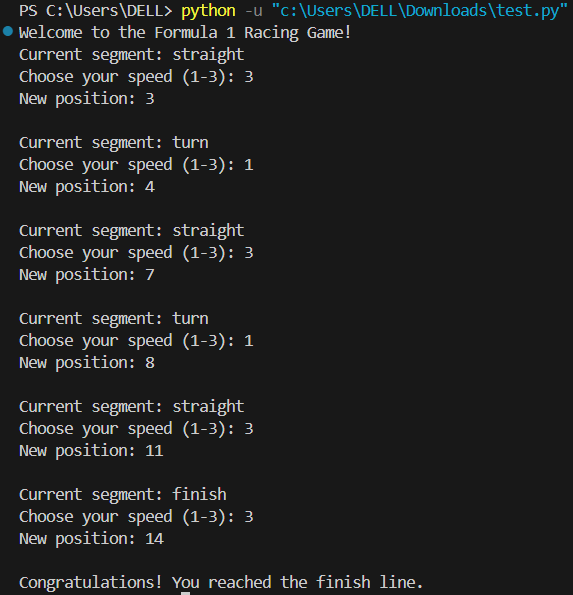
\includegraphics[width=10.5cm]{output2.png}\\
Output for the second scenario
\end{center}
\end{figure}


\section{Analysis and Conclusion}
\subsection{Analysis of Python Functional Programming}
Functional programming in Python, supported through first-class functions, immutability, pure functions, higher-order functions, lambda expressions, and comprehensions, offers a robust paradigm for clean, efficient coding. Emphasizing immutability and pure functions can lead to more predictable and testable code. However, Python's flexibility as a multi-paradigm language means functional programming isn't enforced, allowing for a mix of styles that can either enhance or complicate code consistency. Despite this, integrating functional concepts can significantly improve code quality and maintainability.

\subsection{Conclusion}
The emphasis on immutability and pure functions can lead to more predictable and bug-resistant code, although Python does not enforce immutability strictly. List comprehensions and generator expressions offer elegant solutions for sequence processing, enhancing both readability and performance.\\

% However, Python's flexible and multi-paradigm nature means that it does not enforce a functional programming style. Developers have the freedom to mix functional programming with object-oriented and imperative styles. This flexibility is both a strength and a weakness; it allows for varied approaches to problem-solving but can also lead to less consistent codebases if not managed carefully.\\

In summary, functional programming in Python offers a robust set of tools and practices that can improve code quality and maintainability. While it requires a disciplined approach to fully leverage its benefits, the integration of functional programming concepts into Python's versatile environment can significantly enhance software development outcomes.\\


\begin{thebibliography}{80}

\bibitem{bib1}
Slide theory of Haskell in Ho Chi Minh University of Technology

\bibitem{bib2}
\href{https://positiwise.com/blog/object-oriented-programming-vs-functional-programming-comparison#:~:text=Object%2Doriented%20programming%20focuses%20on,you%20must%20prefer%20functional%20programming.}{Jemin Desai, \textit{Object Oriented Programming vs Functional Programming Comparison}, 2023}

\bibitem{bib3}
\href{https://www.turing.com/kb/introduction-to-functional-programming}{Thulie, \textit{Introduction to Functional Programming}, 2004}

\bibitem{bib4}
\href{https://careers.smartosc.com/en/what-is-python-a-detailed-look-at-this-programming-language/}{SmartOSC, \textit{What is Python? A detailed look at this programming language}, 2000}

\bibitem{bib5}
\href{https://www.freecodecamp.org/news/how-to-setup-virtual-environments-in-python/}{Stephen Sanwo, \textit{How to Set Up a Virtual Environment in Python – And Why It's Useful}, 2022}

\bibitem{bib6}
\href{https://www.formula1.com/}{FIA, \textit{Formula 1}, 1950}

\bibitem{bib7}
\href{https://www.linkedin.com/pulse/functional-programming-game-development-youngjin-kang/}{Youngjin Kang, \textit{Functional Programming for Game Development}, 2023}


\end{thebibliography}
\end{document}